%!TEX root = ../../../adrien_gomar_phd.tex

\subsection{Analysis of the convergence}
\label{sub:dream_hs_steady_conv}

The convergence of the simulation is obtained 
after one thousand iterations for both
the residuals and the similarity coefficients 
(Figure~\ref{fig:dream_HS_convergence_roe2}). More than
five order of magnitude is obtained for the residuals and
the similarity coefficients are stabilized starting below
$1,000$ iterations. According to \citet{Casey2000},
this means that the steady simulation is converged.
\begin{figure}[htp]
  \centering
  \subfigure[residuals]{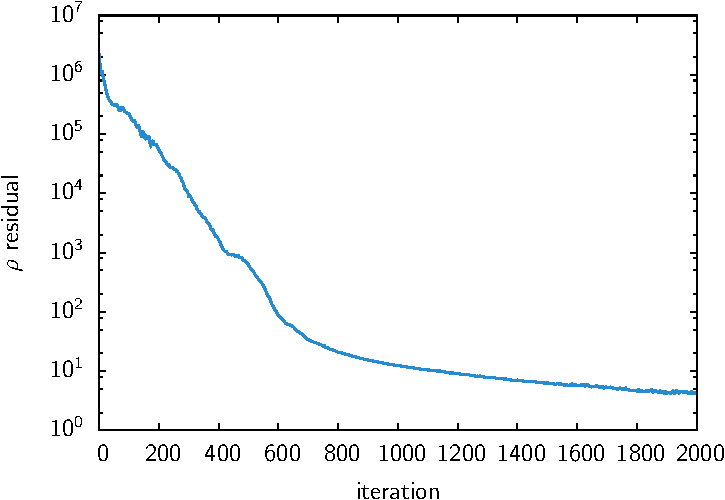
\includegraphics[width=.35\textwidth]{DREAM_HS_RESIDUALS_PPT.pdf}}
  \subfigure[$C_T$]{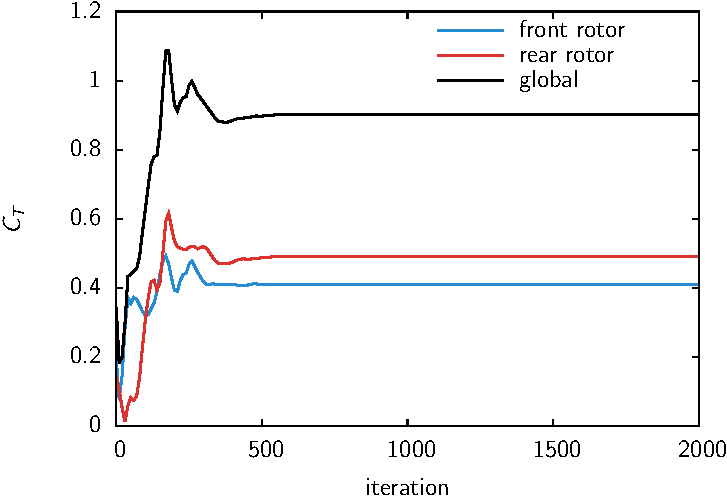
\includegraphics[width=.35\textwidth]{DREAM_HS_FORCES_CT_PPT.pdf}}
  \subfigure[$C_P$]{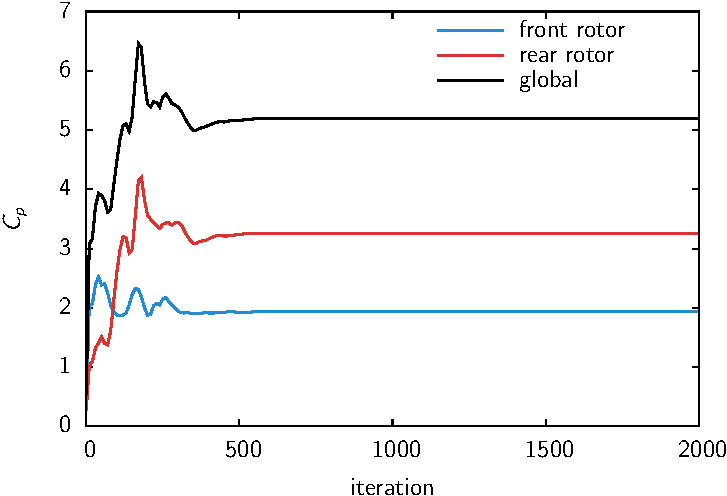
\includegraphics[width=.35\textwidth]{DREAM_HS_FORCES_CP_PPT.pdf}}
  \subfigure[$\eta$]{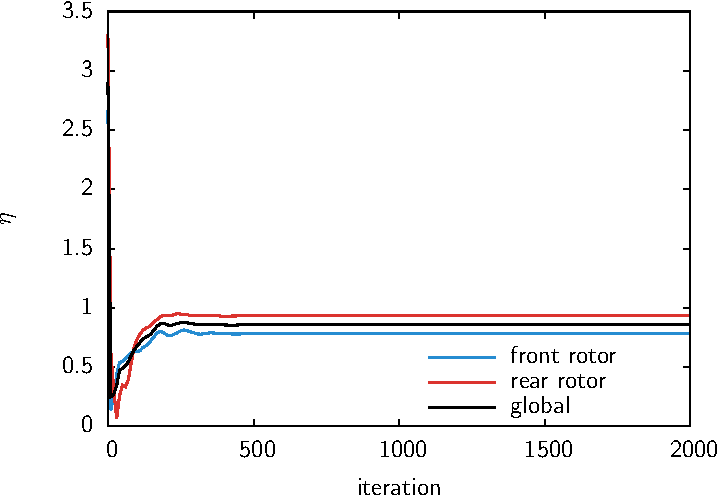
\includegraphics[width=.35\textwidth]{DREAM_HS_FORCES_ETA_PPT.pdf}}
  \caption{High-speed isolated configuration: convergence of the steady
  computation.}
  \label{fig:dream_HS_convergence_roe2}
\end{figure}

\subsection{Similarity coefficients}
\label{sub:dream_hs_sim_coeff}

The similarity coefficients are representative of a cruise
propeller (see Eq.~\eqref{eq:estimation_sim_coeff}). 
Firstly, the thrust is higher
on the rear rotor than on the front rotor, even though it is
relatively well distributed. Bare in mind that the rear rotor
similarity coefficient is normalized by the front rotor diameter. Therefore, 
the thrust produced by the rear rotor is larger than the one of the front rotor, 
relatively to its diameter. 
Secondly, the power coefficient is similar for both the front and the
rear rotor. As the power coefficient represents the mechanical input
given to flow, this means that the mechanical distribution is 
well distributed, which is a design wish.
\begin{table}[htp]
  \ra{1.3} \centering
  \begin{tabular}{ccc|cccccc}
    \toprule
    $C_T$ & $C_P$ & $\eta$ & $C_{T_f}$ & $C_{P_f}$ & $\eta_f$ & $C_{T_r}$ & $C_{P_r}$ & $\eta_r$ \\
    \midrule
    0.9017 & 3.8485 & 0.8577 & 0.4105 & 1.9262 & 0.7801 & 0.4912 & 1.9223 & 0.9354 \\
    \bottomrule
  \end{tabular}
  \caption{High-speed isolated configuration: similarity coefficients.}
  \label{tab:dream_HS_sim_coeff}
\end{table}

\subsection{Radial profiles}
\label{sub:dream_hs_radial_profiles}

Radial profiles are computed on the steady results and 
reported in Fig.~\ref{fig:dream_HS_radial_profiles}.

The absolute Mach number increases from its inflow
value ($M_a = 0.73$) up to around $M_a=0.81$. This represents
a 10\% increase that has to be compared to the 100\% increase
for the low-speed configuration. The stream tube contraction
is barely seen as the increase in velocity remains bounded.
It seems that the front rotor tip vortices do not interact
with the rear rotor blades as the small increase near 90\%
of the span, which is attributed to the core of the vortices,
is not contracted by the stream tube.

The absolute angle of the velocity highlights, again, the advantage
of using a CROR compared to a single row propeller system. In fact,
the flow is deviated by the front rotor from its axial direction
to a mean $5^\circ$ velocity vector. The rear rotor then deviates
back the flow field to make it almost purely axial with exceptions
near the hub and near the front tip vortex region ($0.75 \leq R/R_f \leq 0.95$).
This finally explains the efficiency of a CROR propeller system.

Compared to a 

\begin{figure}[htp]
  \centering
  \subfigure[absolute Mach number]{
    \label{fig:dream_HS_radial_profiles_ma}
    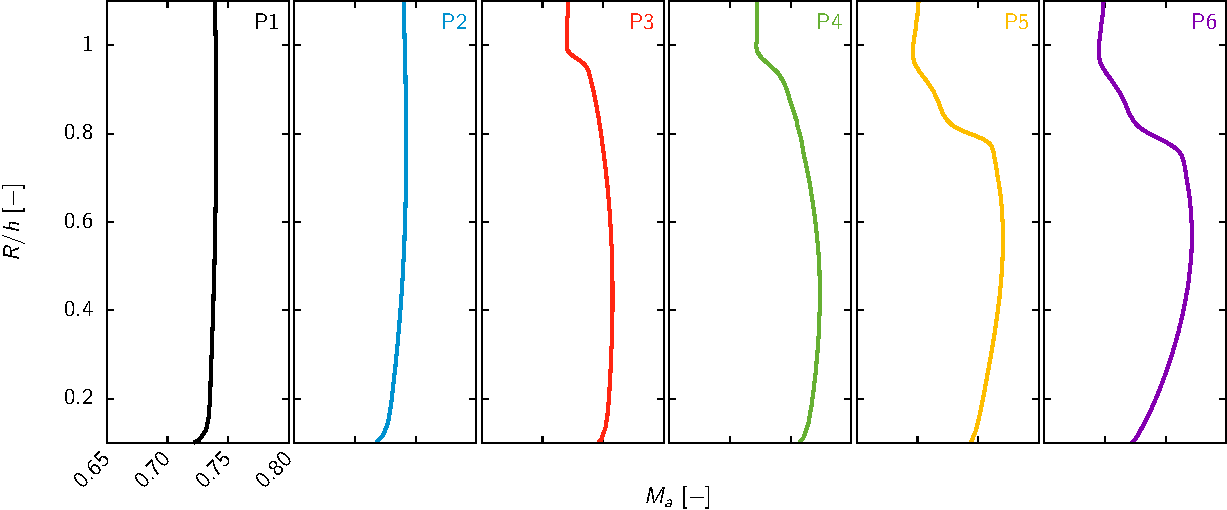
\includegraphics[width=.72\textwidth]{DREAM_HS_RANS_AZI_MEAN_PPT_macha.pdf}}
  \subfigure[absolute flow angle]{
    \label{fig:dream_HS_radial_profiles_alpha}
    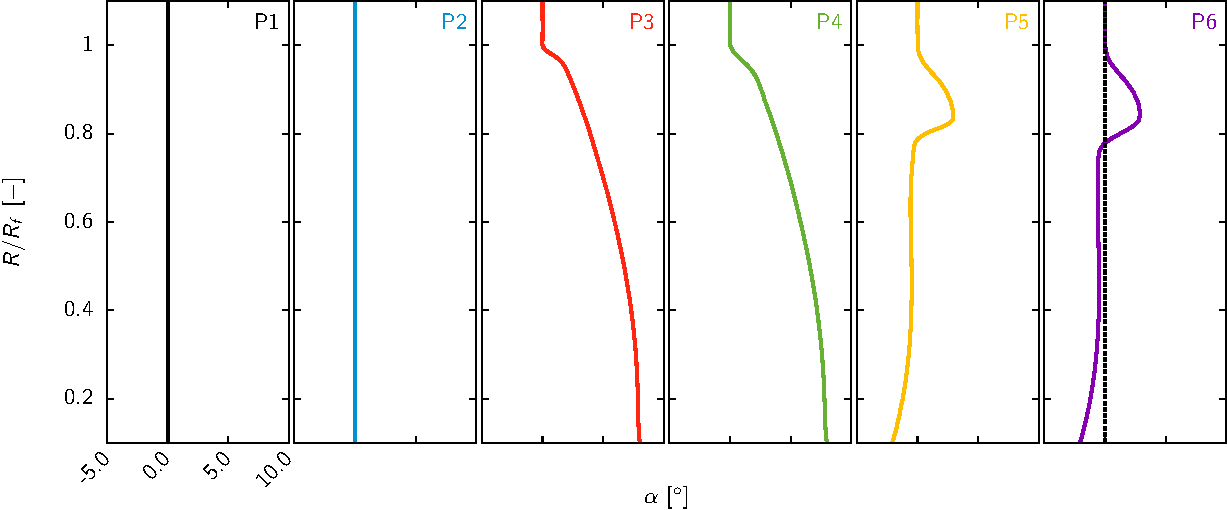
\includegraphics[width=.72\textwidth]{DREAM_HS_RANS_AZI_MEAN_PPT_alpha.pdf}}
  \caption{High-speed isolated configuration: radial profiles.}
\end{figure}
\setcounter{figure}{\value{figure}-1}
\begin{figure}[htp]
  \centering
  \setcounter{subfigure}{3}
  \subfigure[static pressure]{
    \label{fig:dream_HS_radial_profiles_ps}
    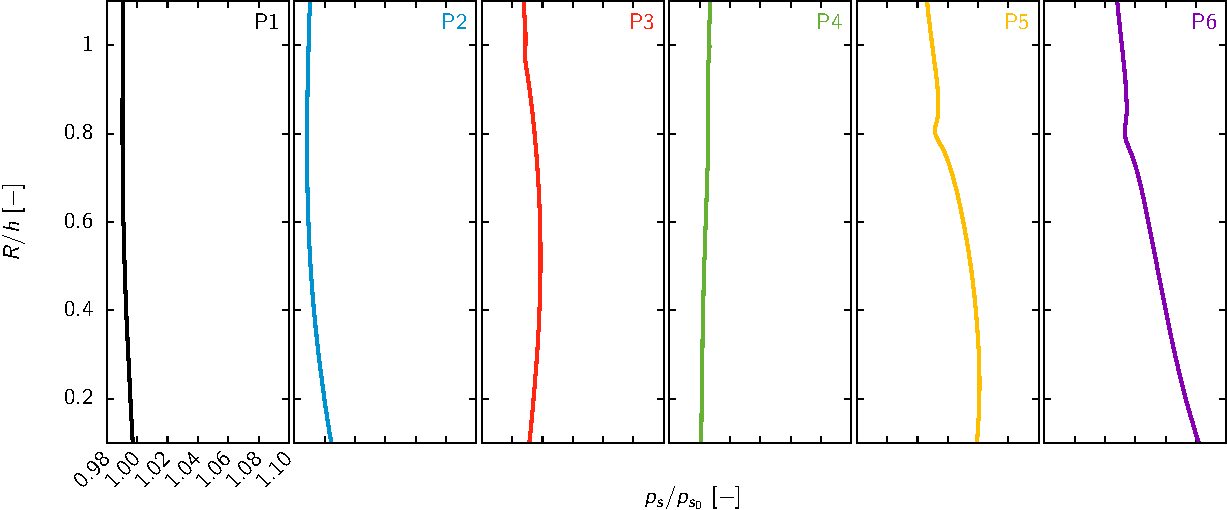
\includegraphics[width=.72\textwidth]{DREAM_HS_RANS_AZI_MEAN_PPT_ps.pdf}}
  \subfigure[stagnation pressure]{
    \label{fig:dream_HS_radial_profiles_pi}
    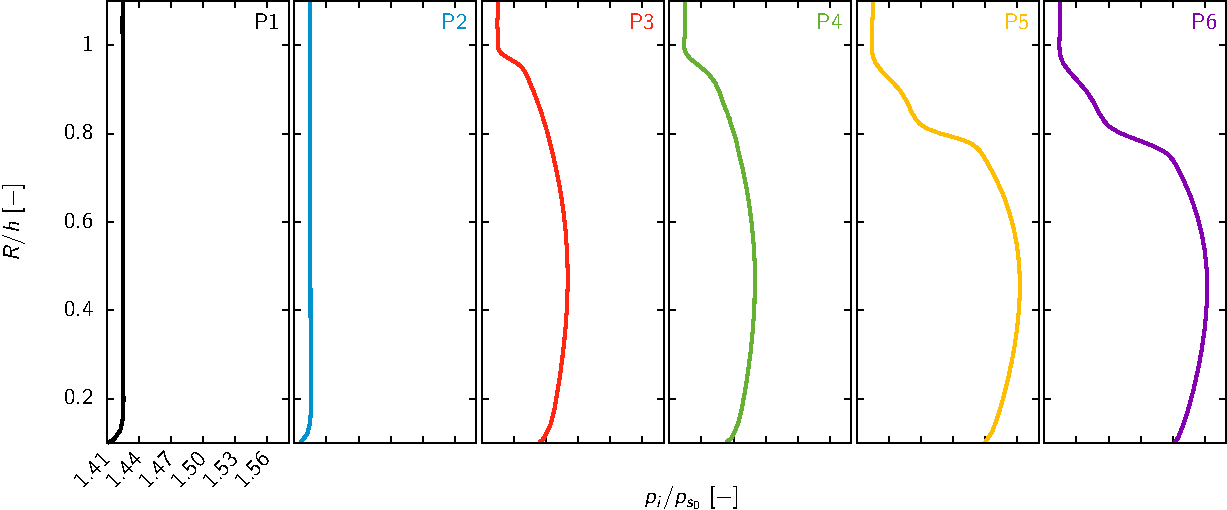
\includegraphics[width=.72\textwidth]{DREAM_HS_RANS_AZI_MEAN_PPT_pi.pdf}}
  \subfigure[stagnation temperature]{
    \label{fig:dream_HS_radial_profiles_ti}
    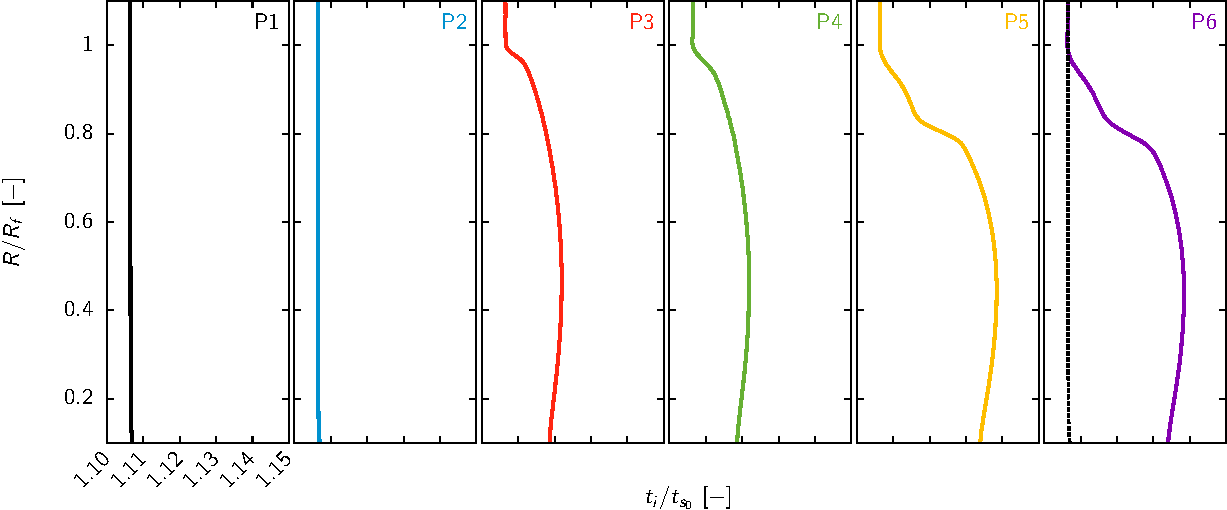
\includegraphics[width=.72\textwidth]{DREAM_HS_RANS_AZI_MEAN_PPT_ti.pdf}}
  \caption{High-speed isolated configuration: radial profiles (contd.).}
  \label{fig:dream_HS_radial_profiles}
\end{figure}

\subsection{Flow field around the blades}
\label{sub:dream_hs_blades}


\begin{figure}[htp]
 \centering
 \begin{tabular}{rccc}
   & $-k_p$ front rotor
   & $-k_p$ rear rotor
   & relative Mach number\\
   \rotatebox{90}{\qquad\qquad 25~\%} 
   & 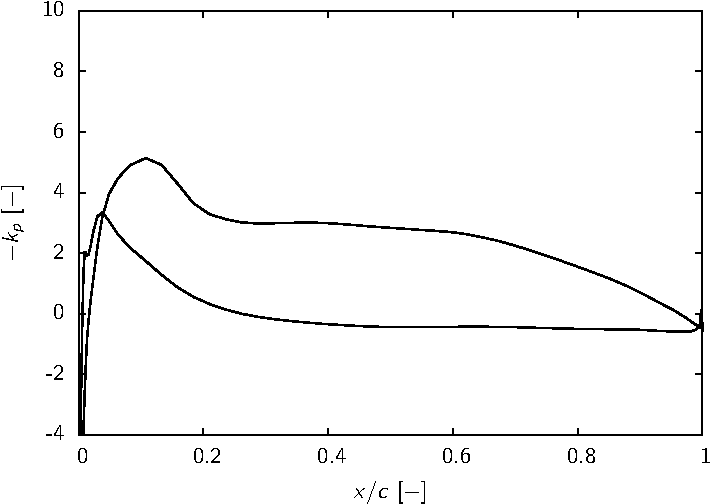
\includegraphics[width=0.28\textwidth]{DREAM_HS_KP_25_FRONT_PPT.pdf}
   & 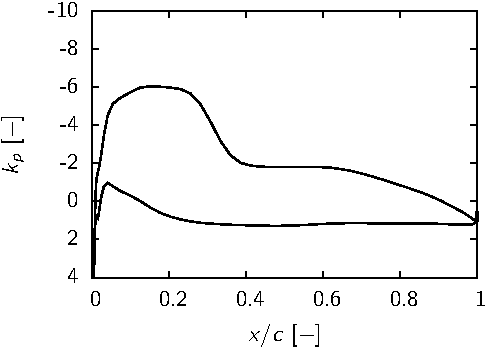
\includegraphics[width=0.28\textwidth]{DREAM_HS_KP_25_REAR_PPT.pdf}
   & 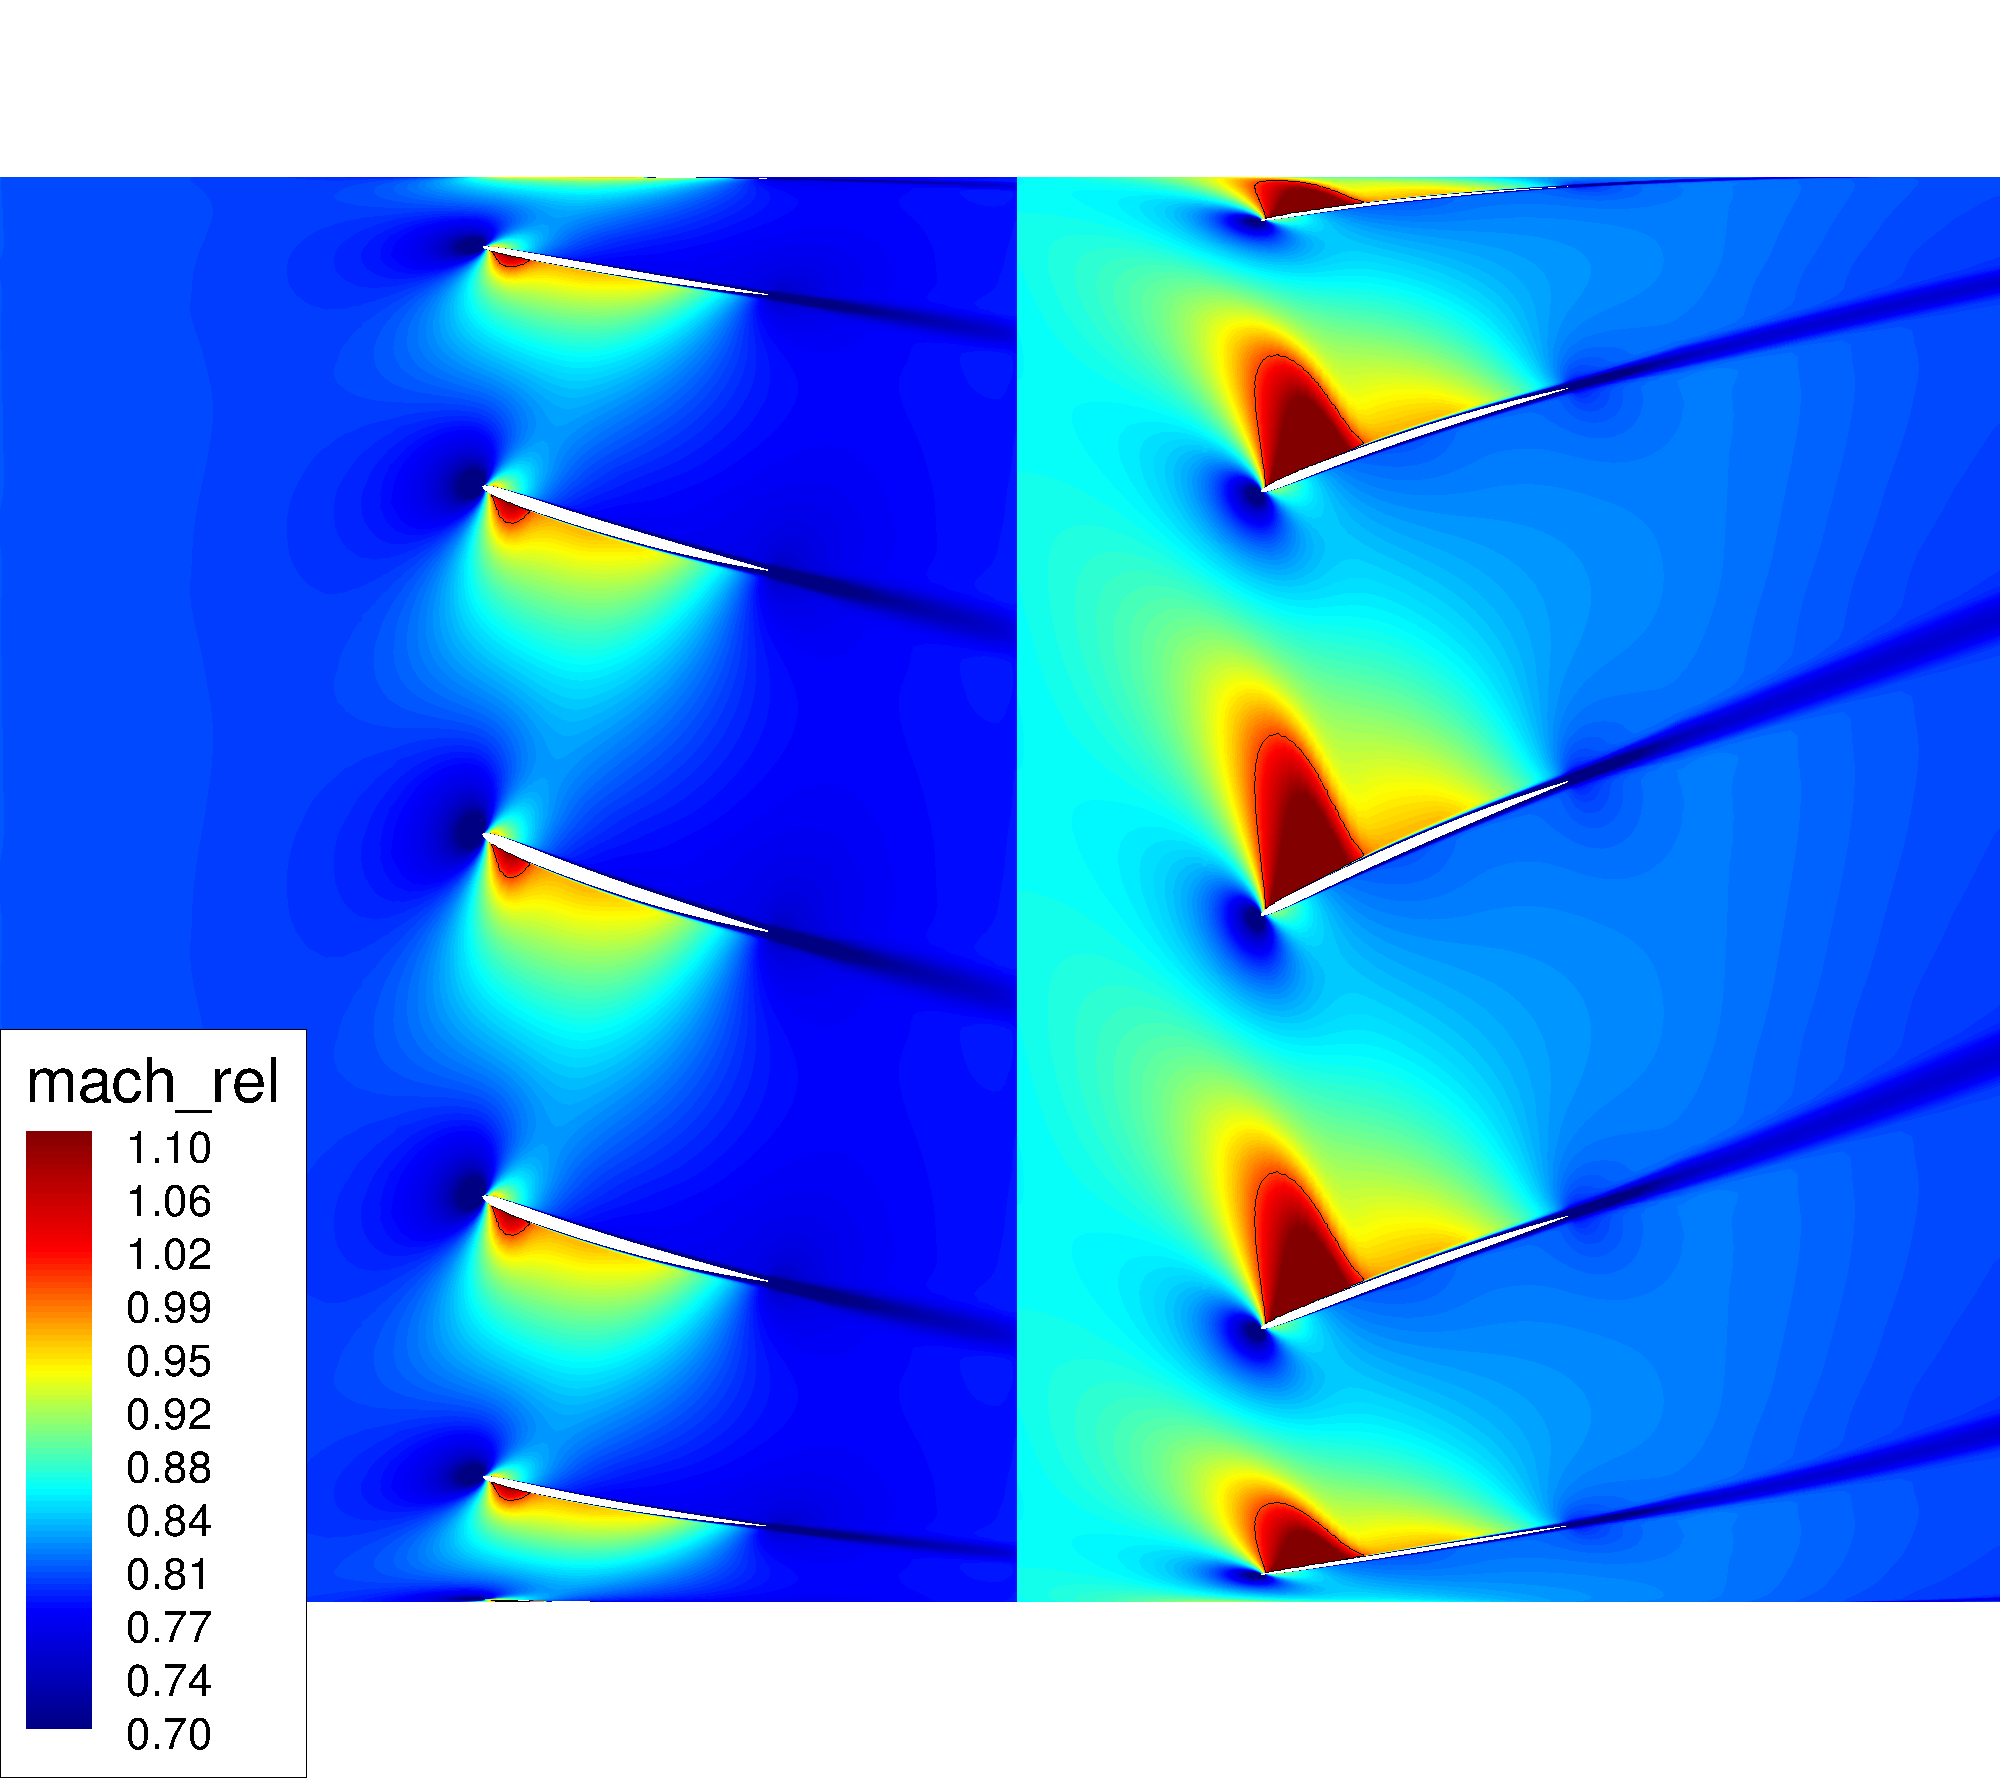
\includegraphics[width=0.28\textwidth]{DREAM_HS_RANS_roe2_sa_slice_r_25_mach_rel.png}\\
   \rotatebox{90}{\qquad\qquad 50~\%} 
   & 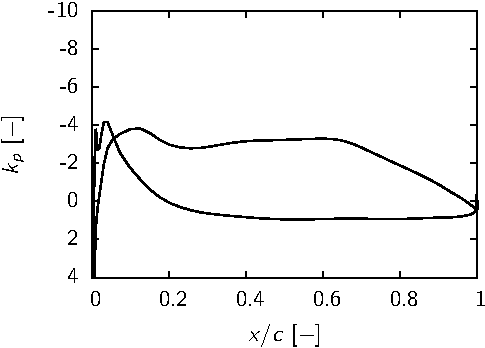
\includegraphics[width=0.28\textwidth]{DREAM_HS_KP_50_FRONT_PPT.pdf}
   & 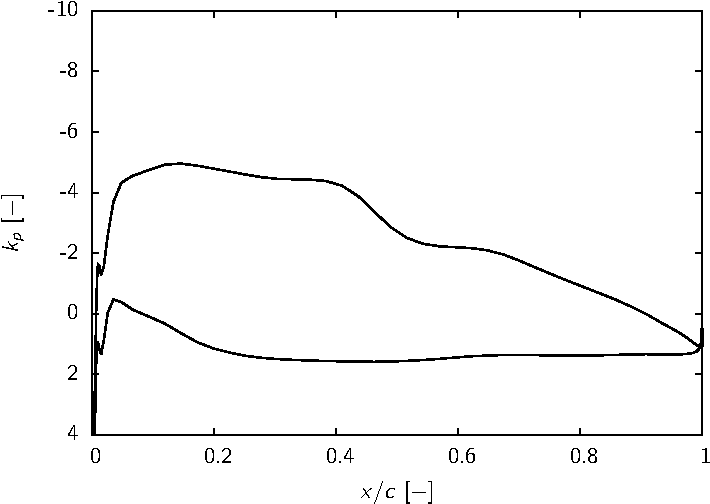
\includegraphics[width=0.28\textwidth]{DREAM_HS_KP_50_REAR_PPT.pdf}
   & 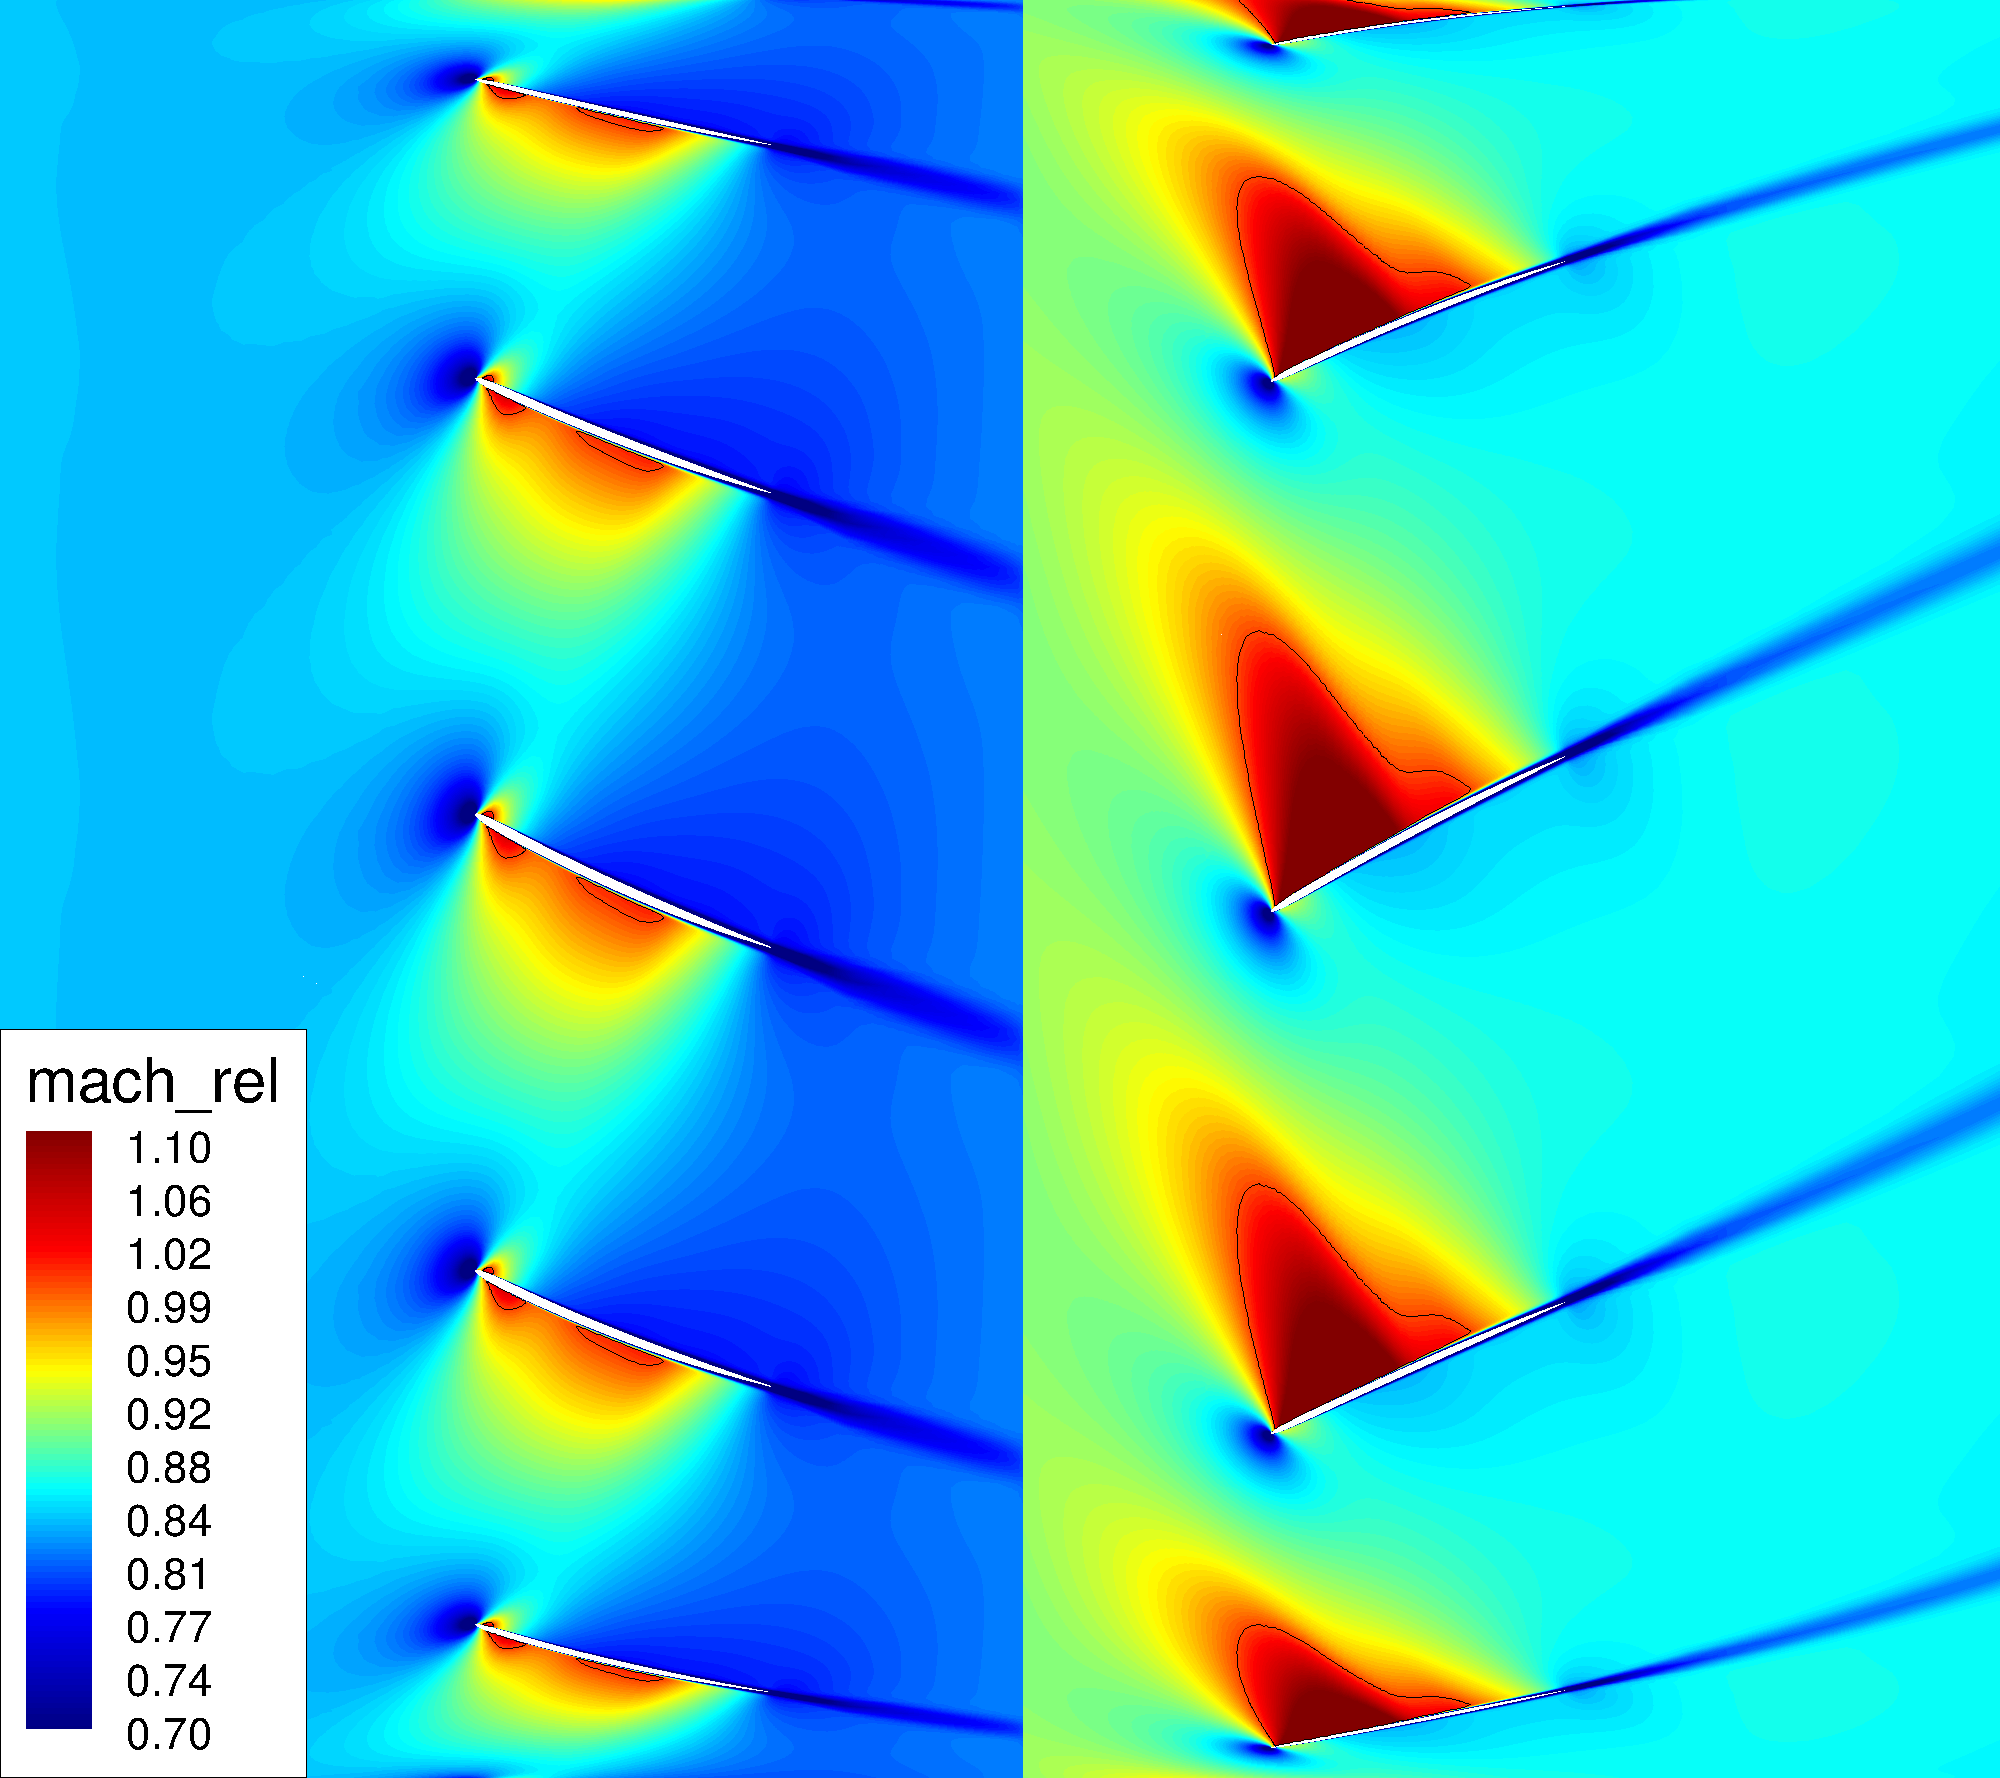
\includegraphics[width=0.28\textwidth]{DREAM_HS_RANS_roe2_sa_slice_r_50_mach_rel.png}\\
   \rotatebox{90}{\qquad\qquad 75~\%} 
   & 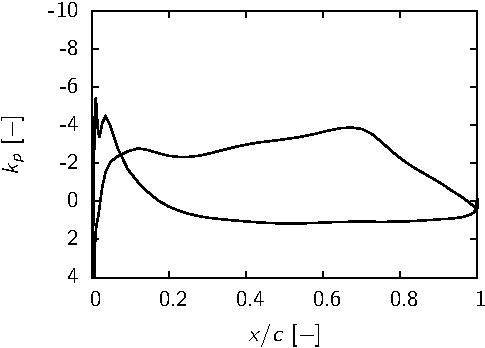
\includegraphics[width=0.28\textwidth]{DREAM_HS_KP_75_FRONT_PPT.pdf}
   & 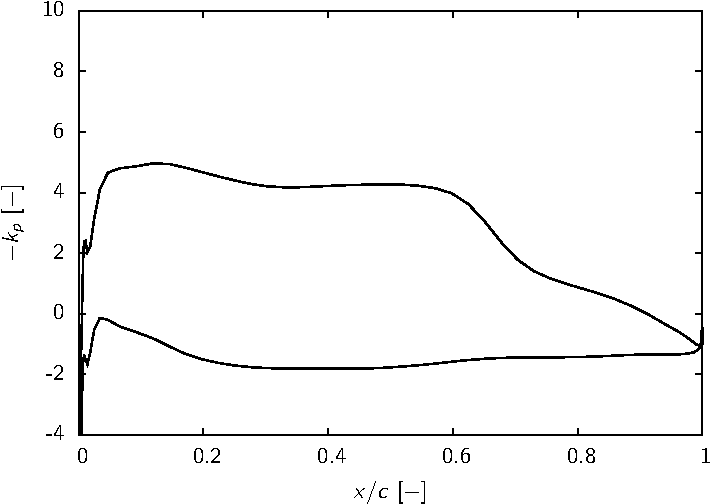
\includegraphics[width=0.28\textwidth]{DREAM_HS_KP_75_REAR_PPT.pdf}
   & 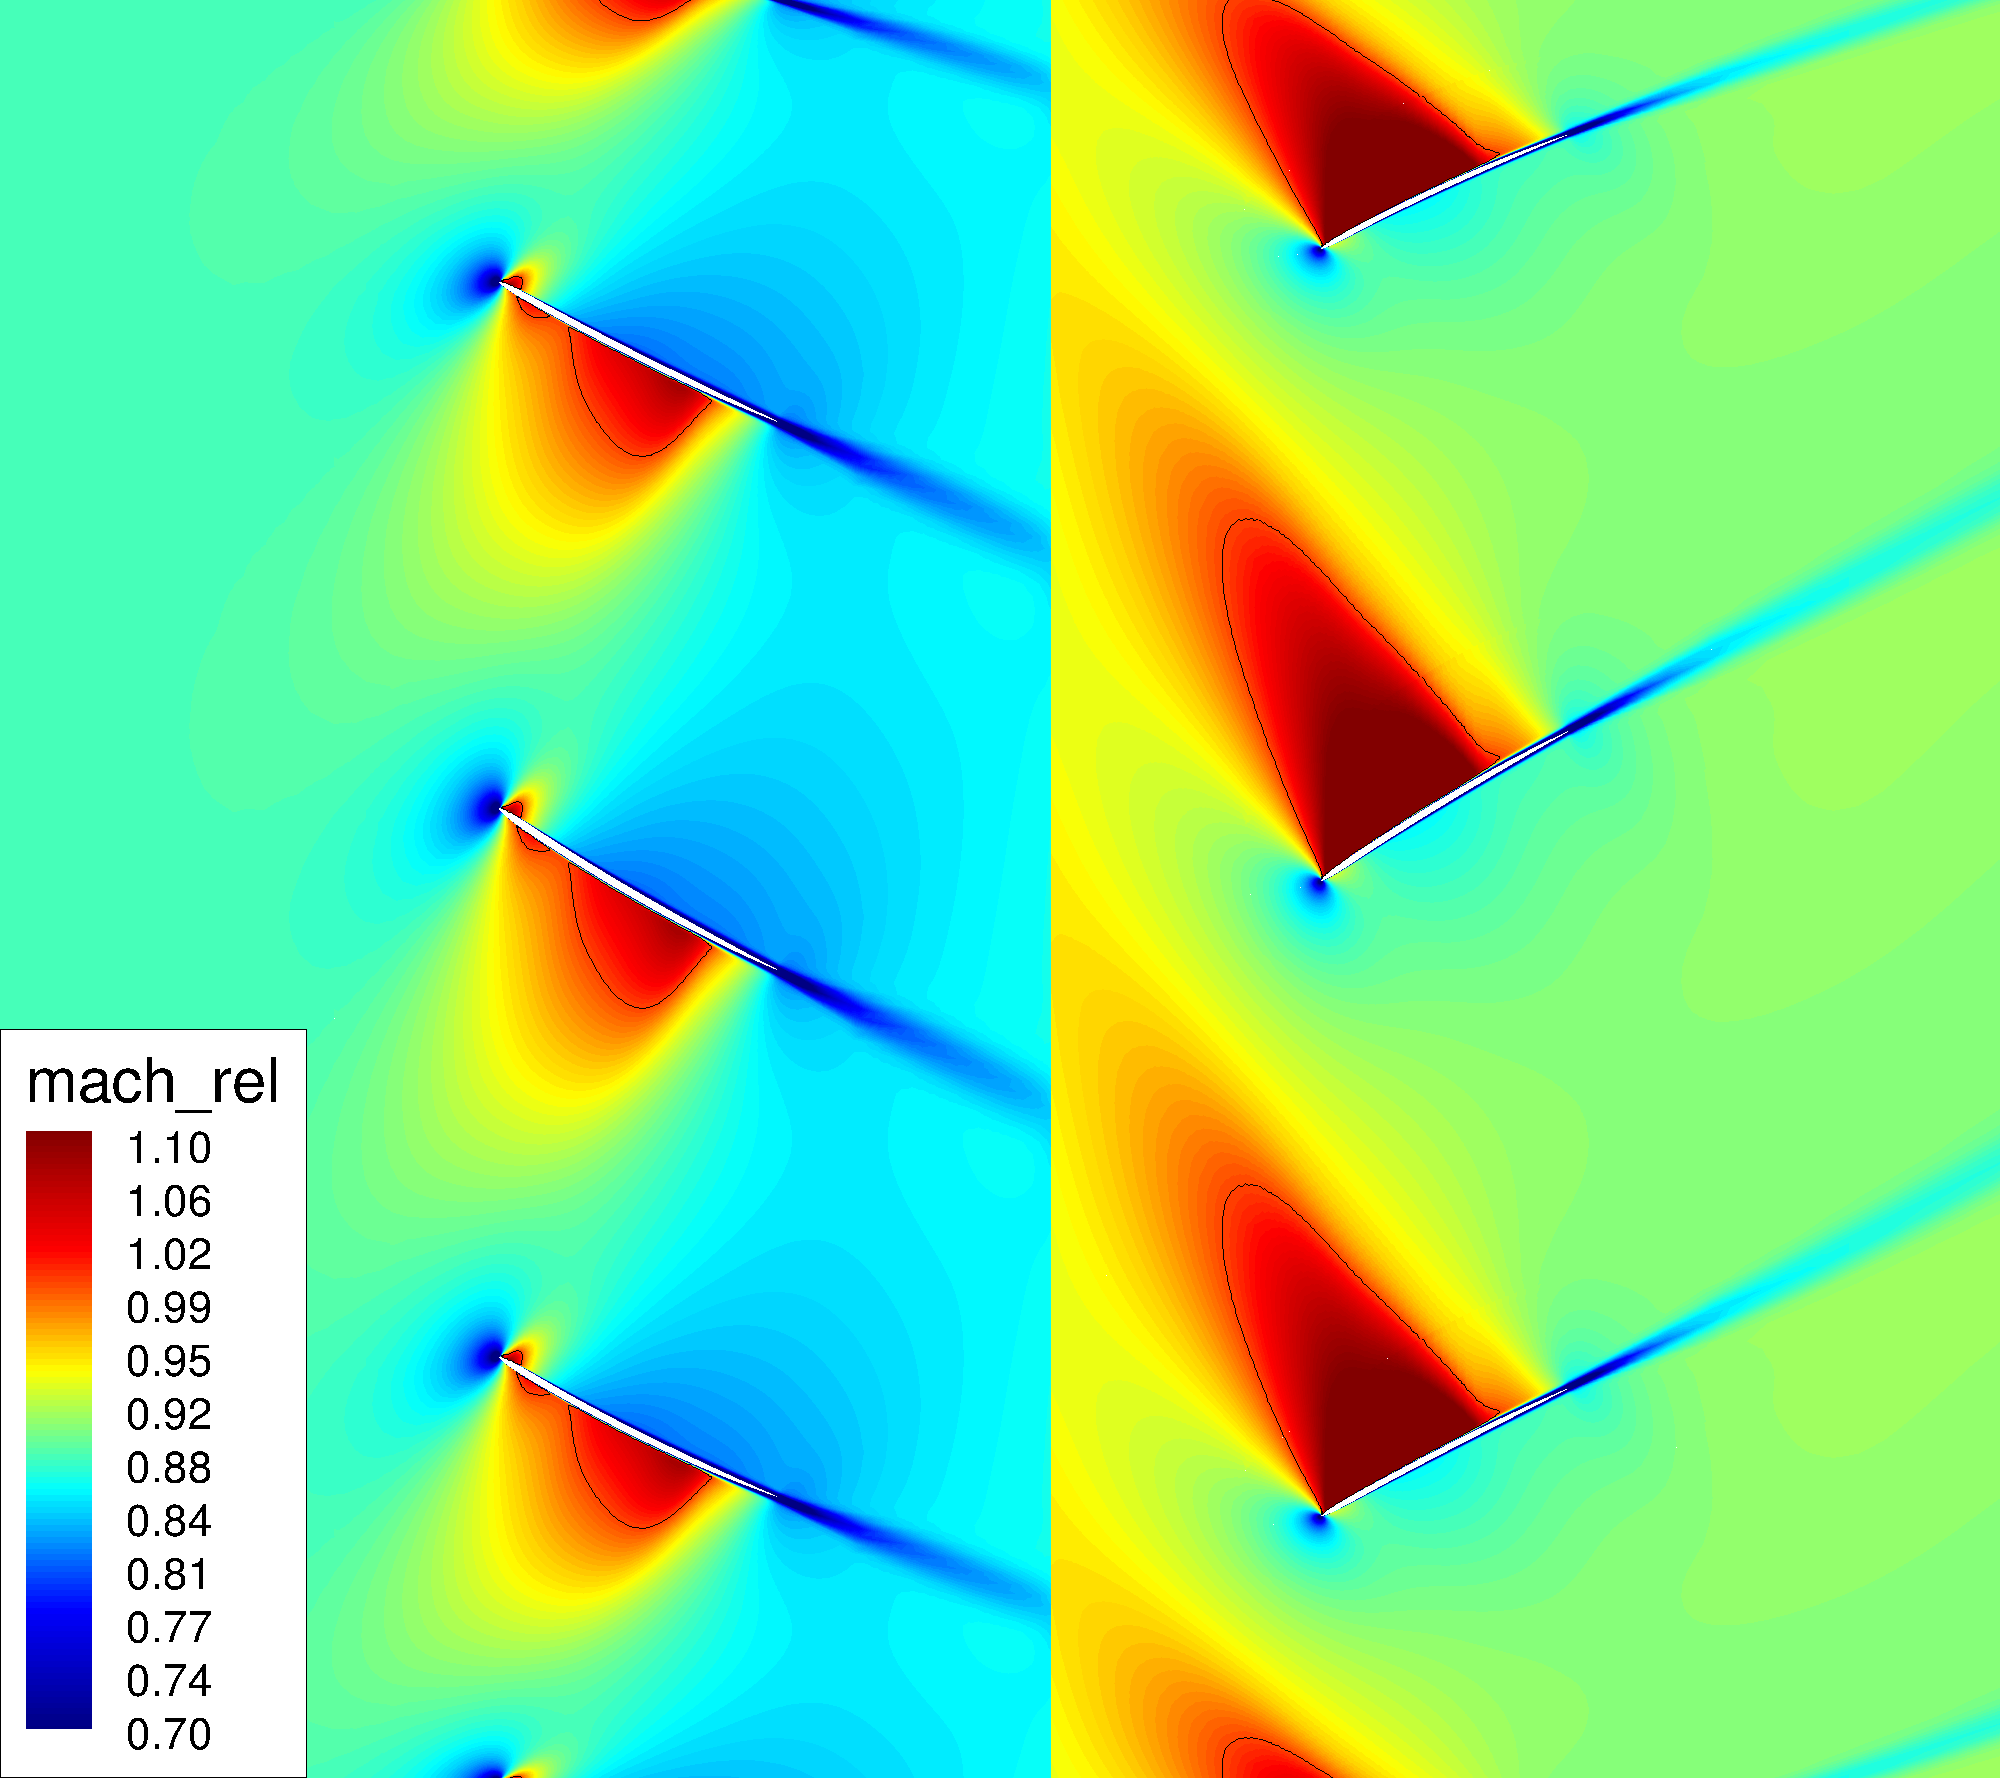
\includegraphics[width=0.28\textwidth]{DREAM_HS_RANS_roe2_sa_slice_r_75_mach_rel.png}\\
   \rotatebox{90}{\qquad\qquad 90~\%} 
   & 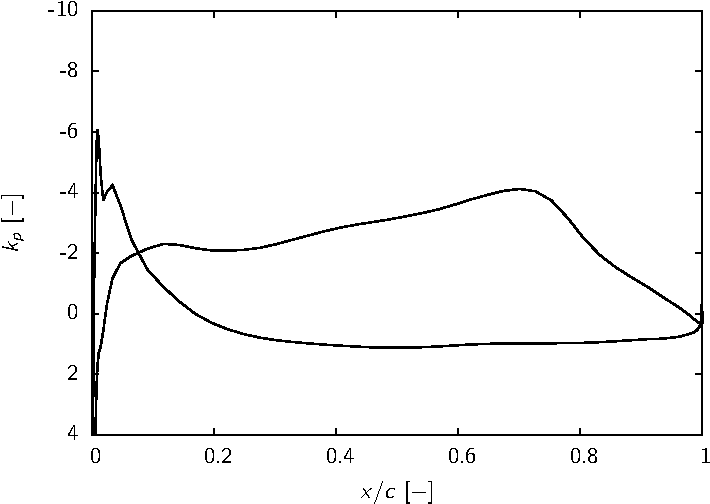
\includegraphics[width=0.28\textwidth]{DREAM_HS_KP_90_FRONT_PPT.pdf}
   & 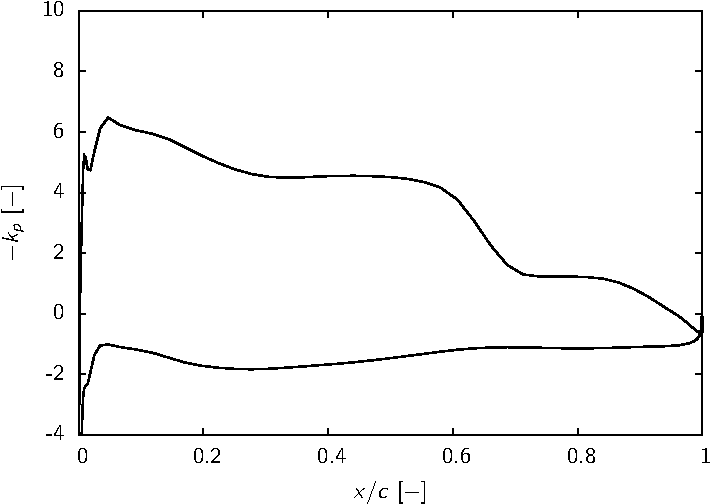
\includegraphics[width=0.28\textwidth]{DREAM_HS_KP_90_REAR_PPT.pdf}
   & 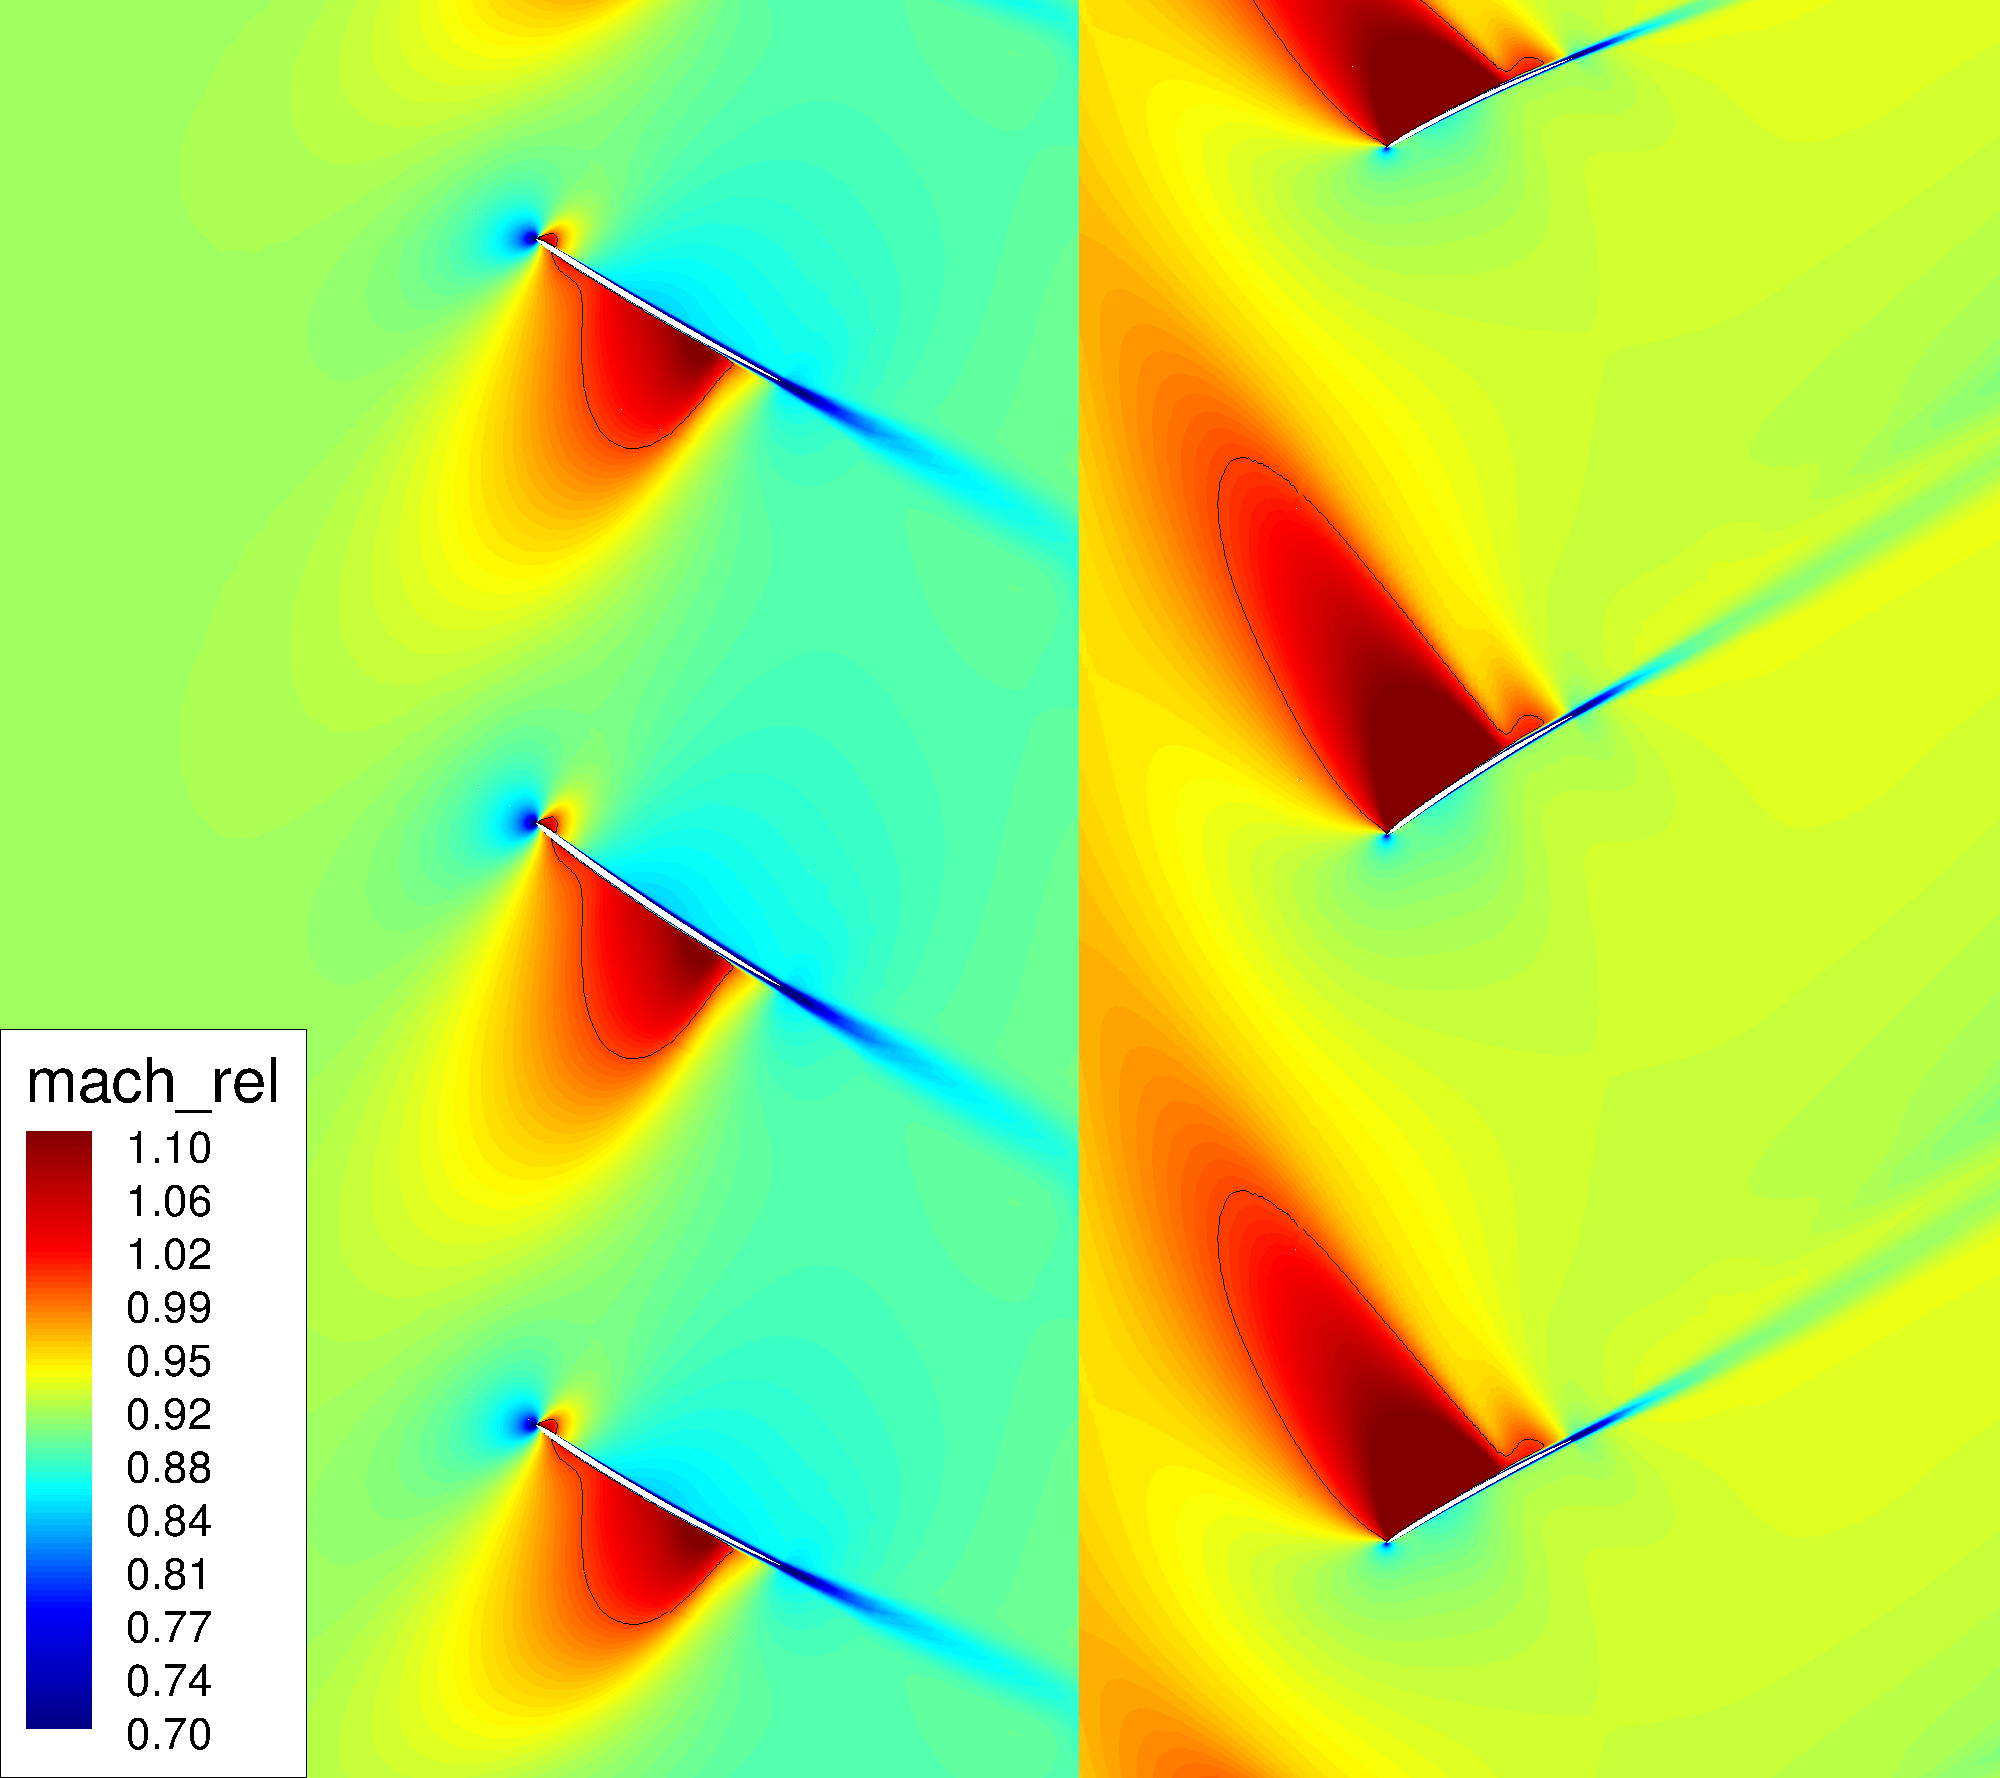
\includegraphics[width=0.28\textwidth]{DREAM_HS_RANS_roe2_sa_slice_r_90_mach_rel.png}\\
   \rotatebox{90}{\qquad\qquad 95~\%} 
   & 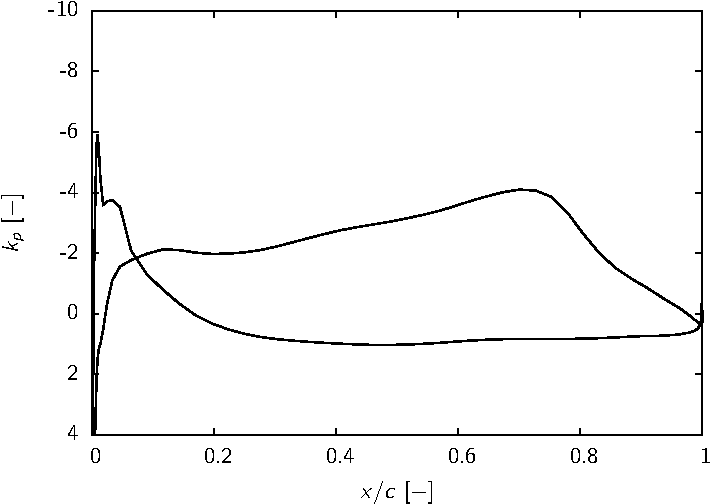
\includegraphics[width=0.28\textwidth]{DREAM_HS_KP_95_FRONT_PPT.pdf}
   & 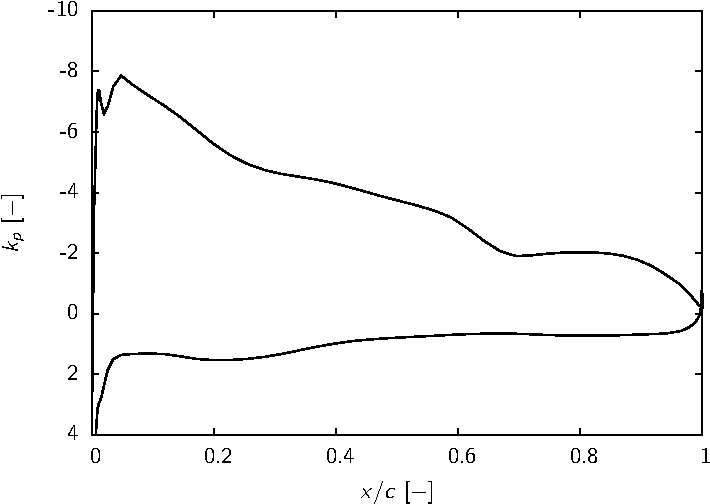
\includegraphics[width=0.28\textwidth]{DREAM_HS_KP_95_REAR_PPT.pdf}
   & 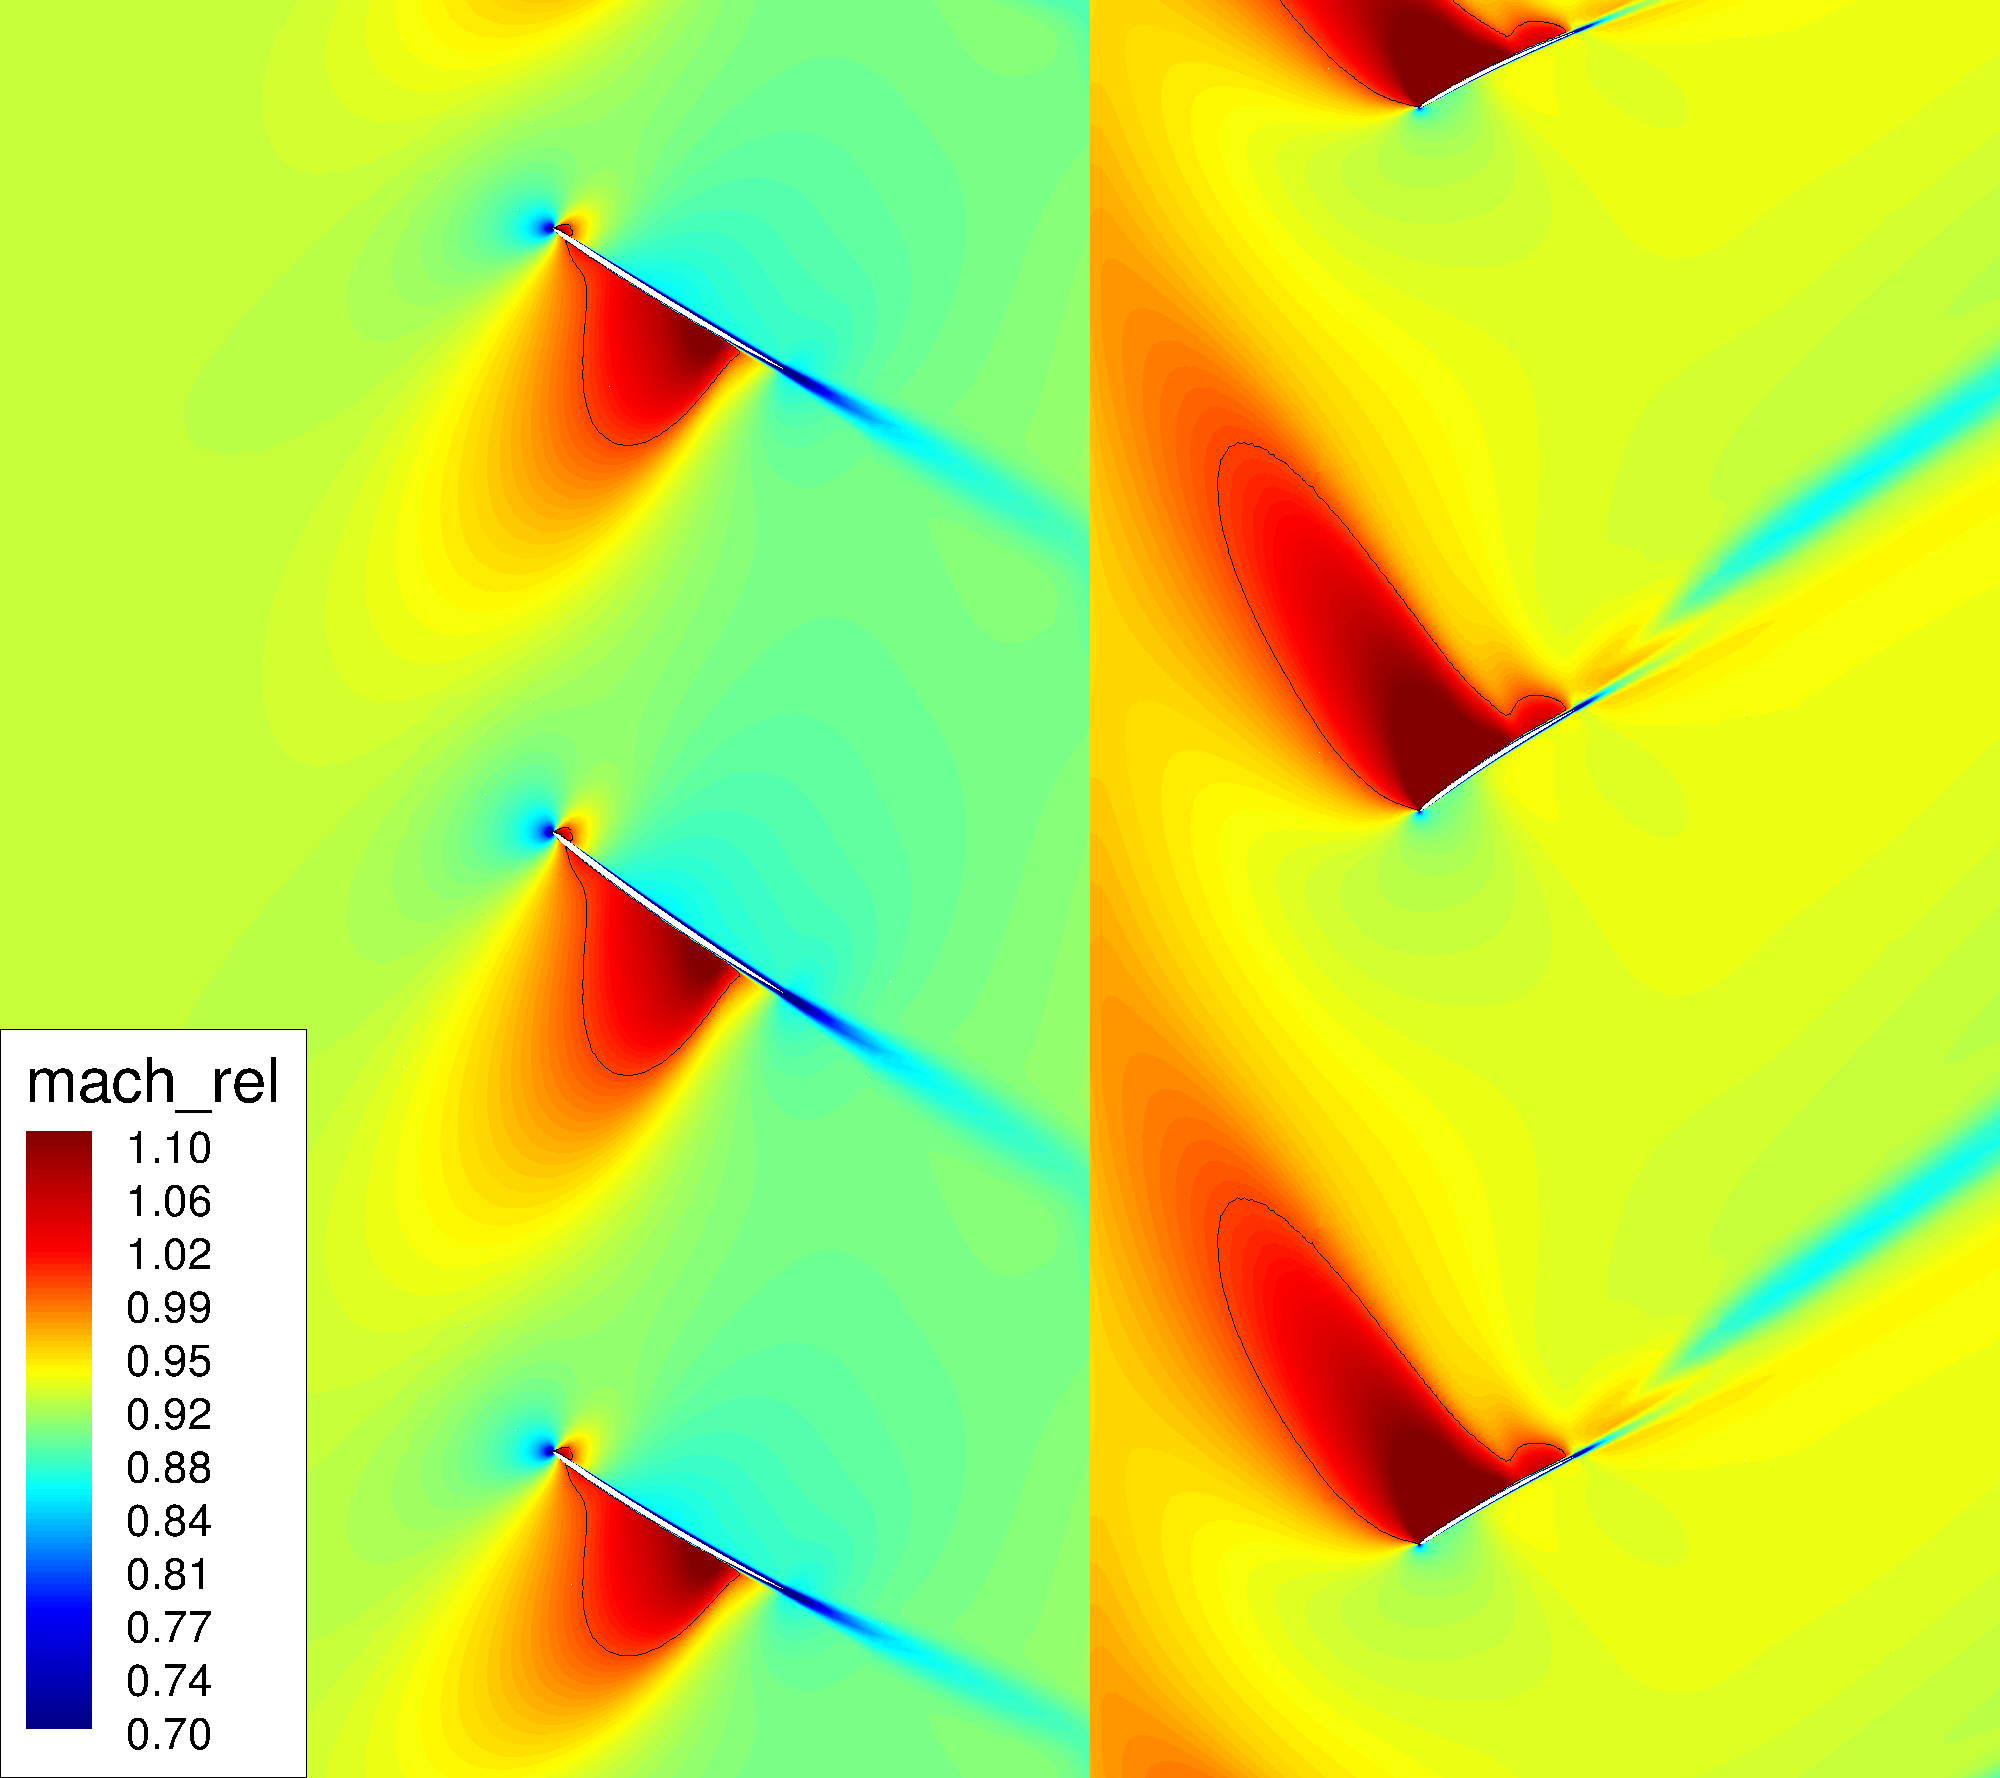
\includegraphics[width=0.28\textwidth]{DREAM_HS_RANS_roe2_sa_slice_r_95_mach_rel.png}  
 \end{tabular}
 \caption{High-speed isolated configuration: pressure coefficient and relative Mach
 number contours at different radial position.}
 \label{fig:dream_HS_mach_kp}
\end{figure}

\begin{figure}[htp]
  \centering
  \subfigure[$P3$]{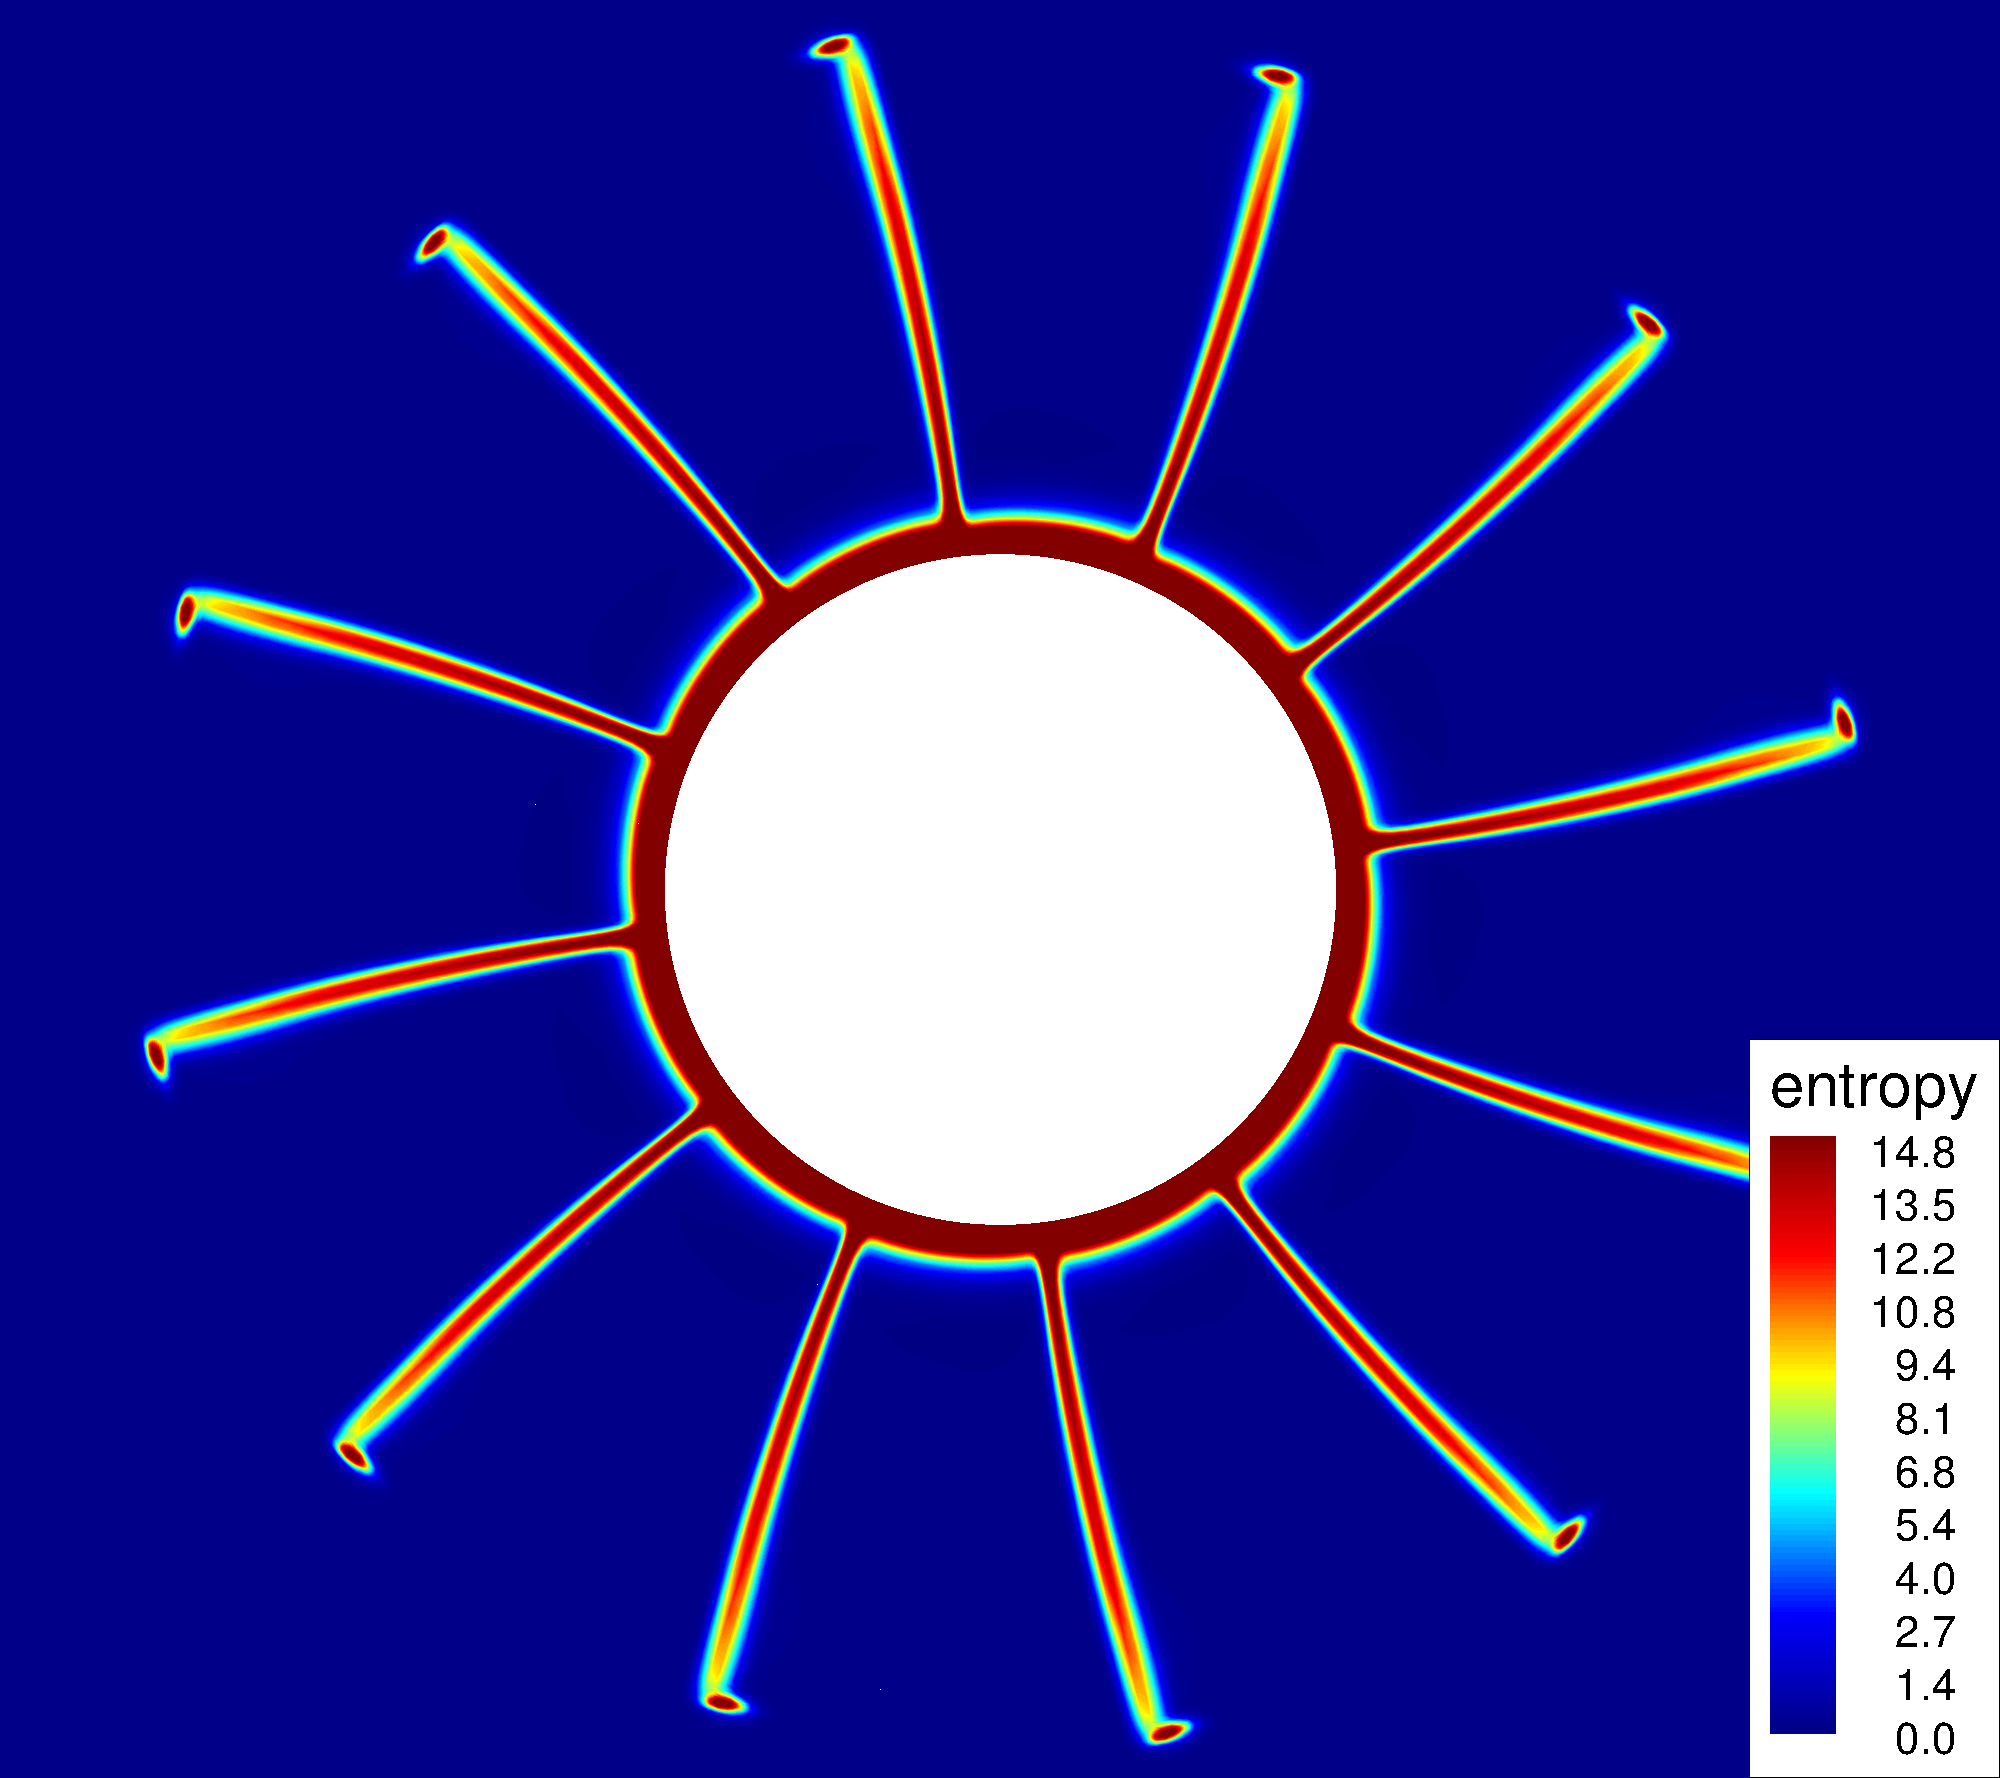
\includegraphics[width=.35\textwidth]{DREAM_HS_RANS_roe2_sa_slice_x_front_1_entropy.png}}
  \subfigure[$P4$]{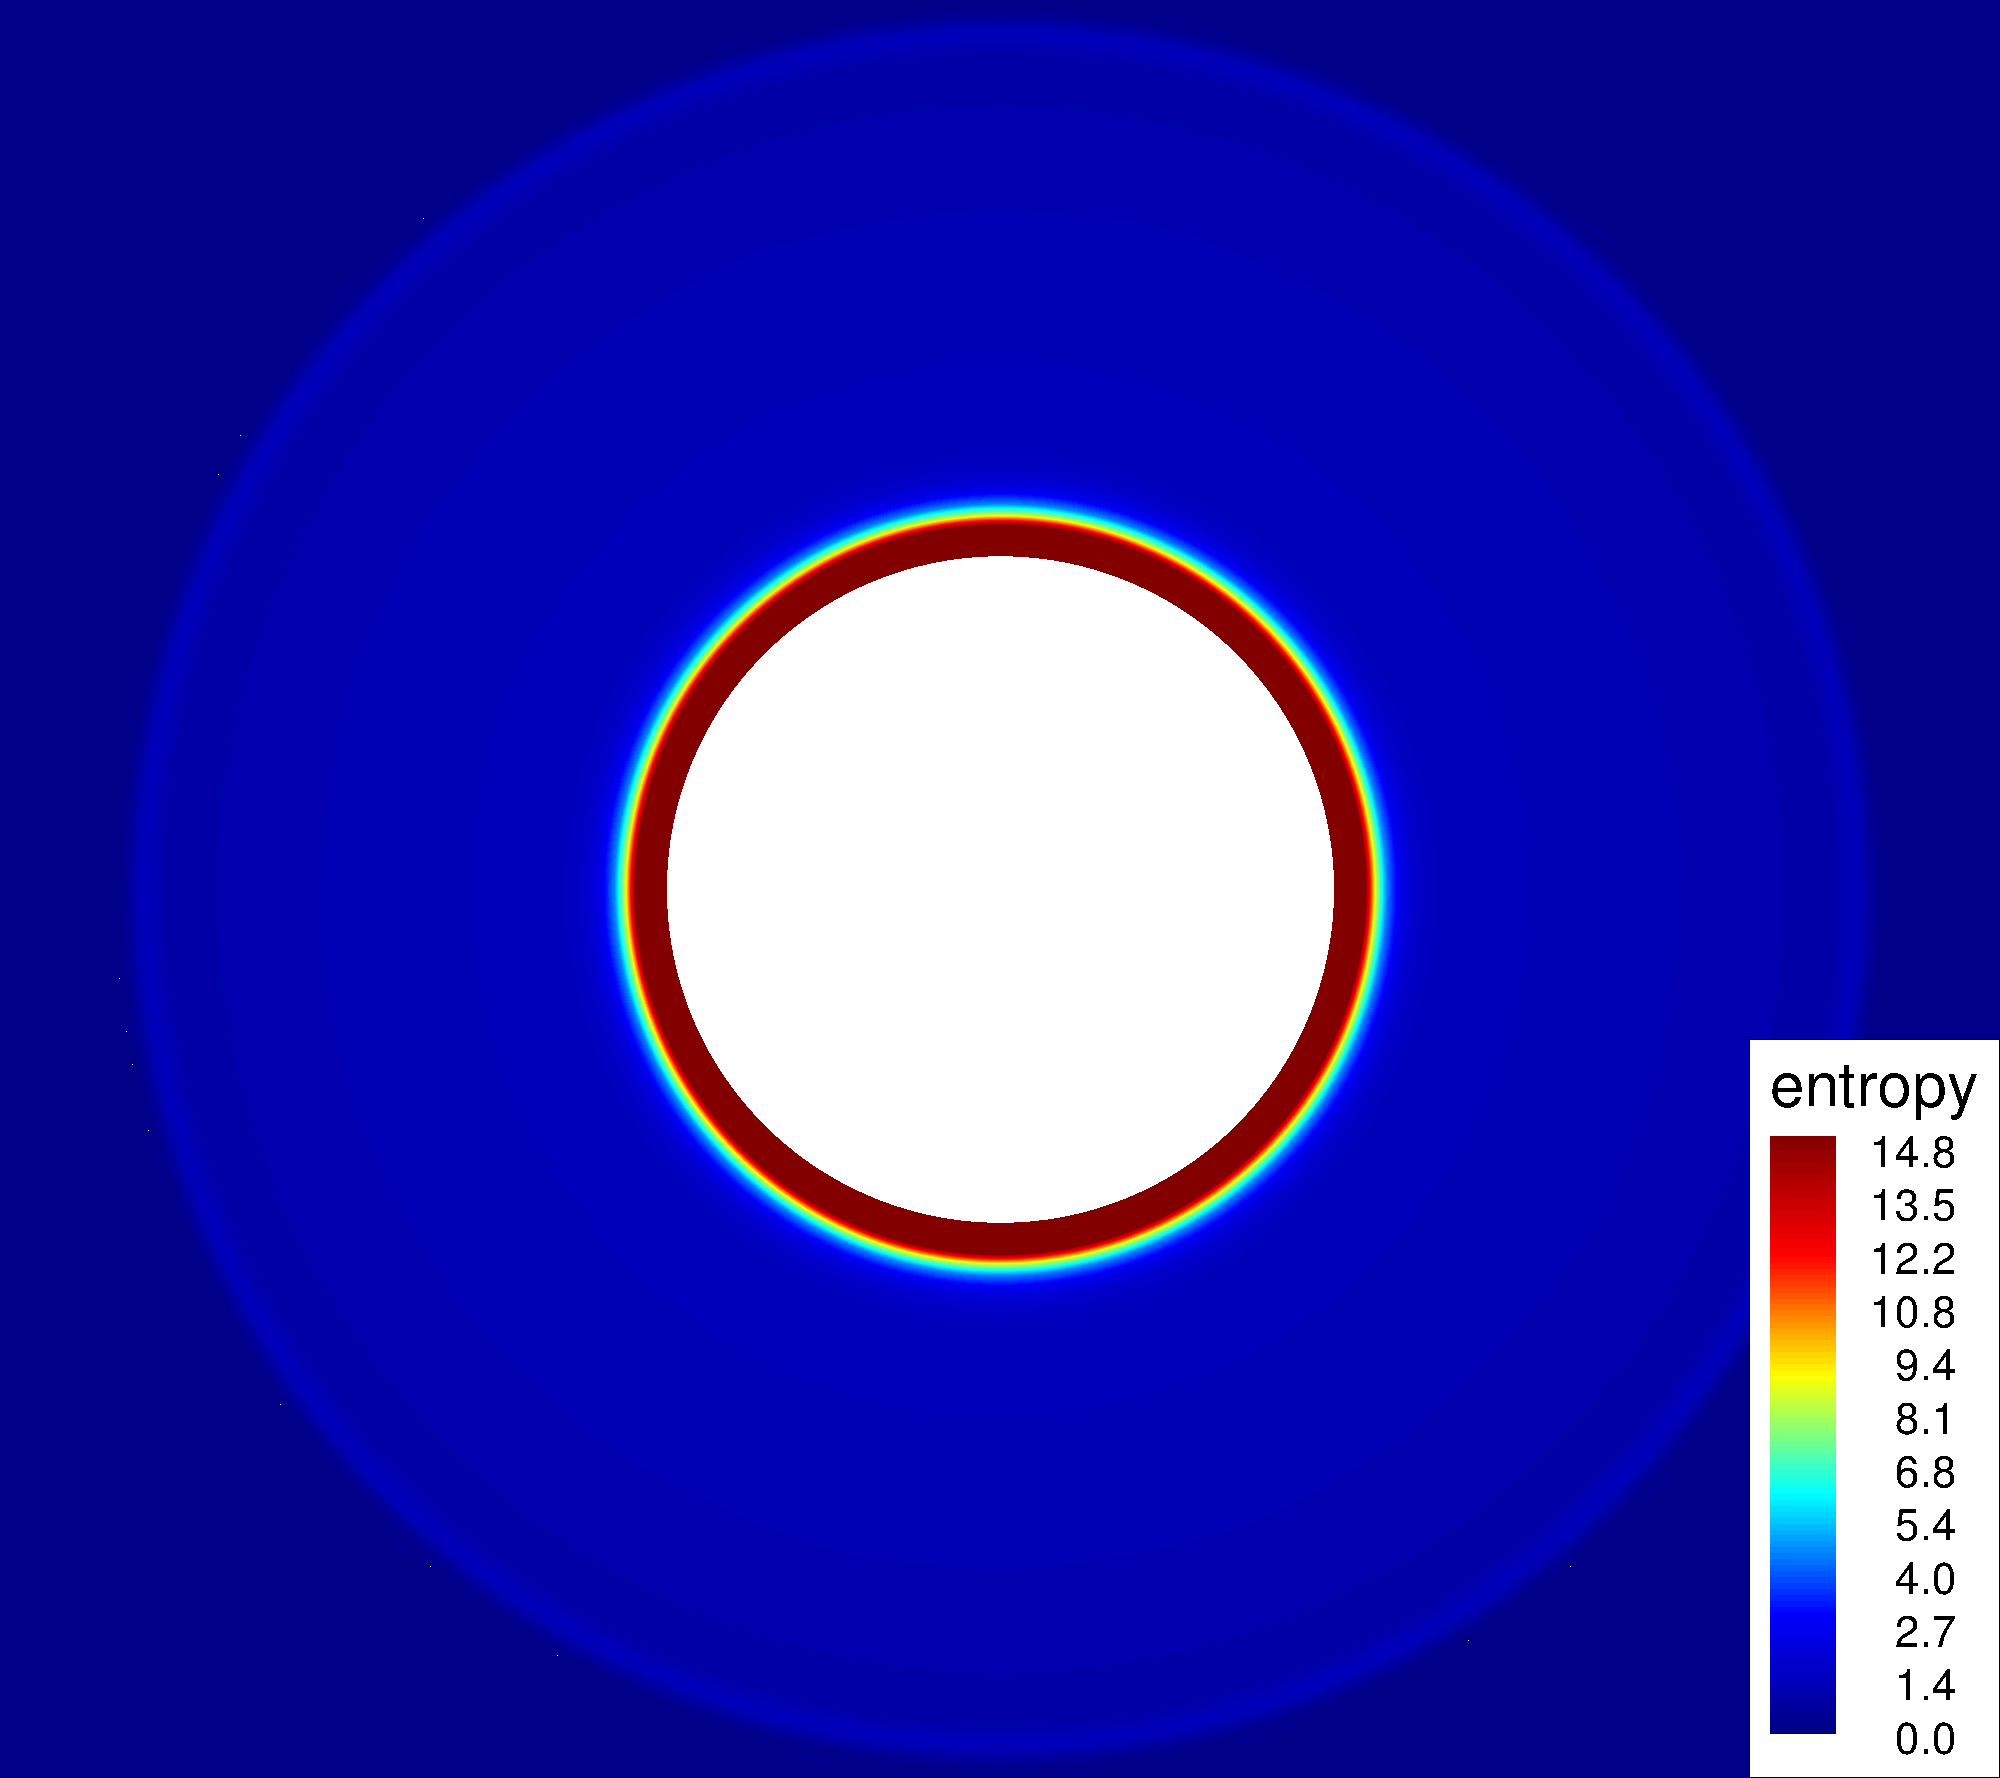
\includegraphics[width=.35\textwidth]{DREAM_HS_RANS_roe2_sa_slice_x_rear_0_entropy.png}}
  \subfigure[$P5$]{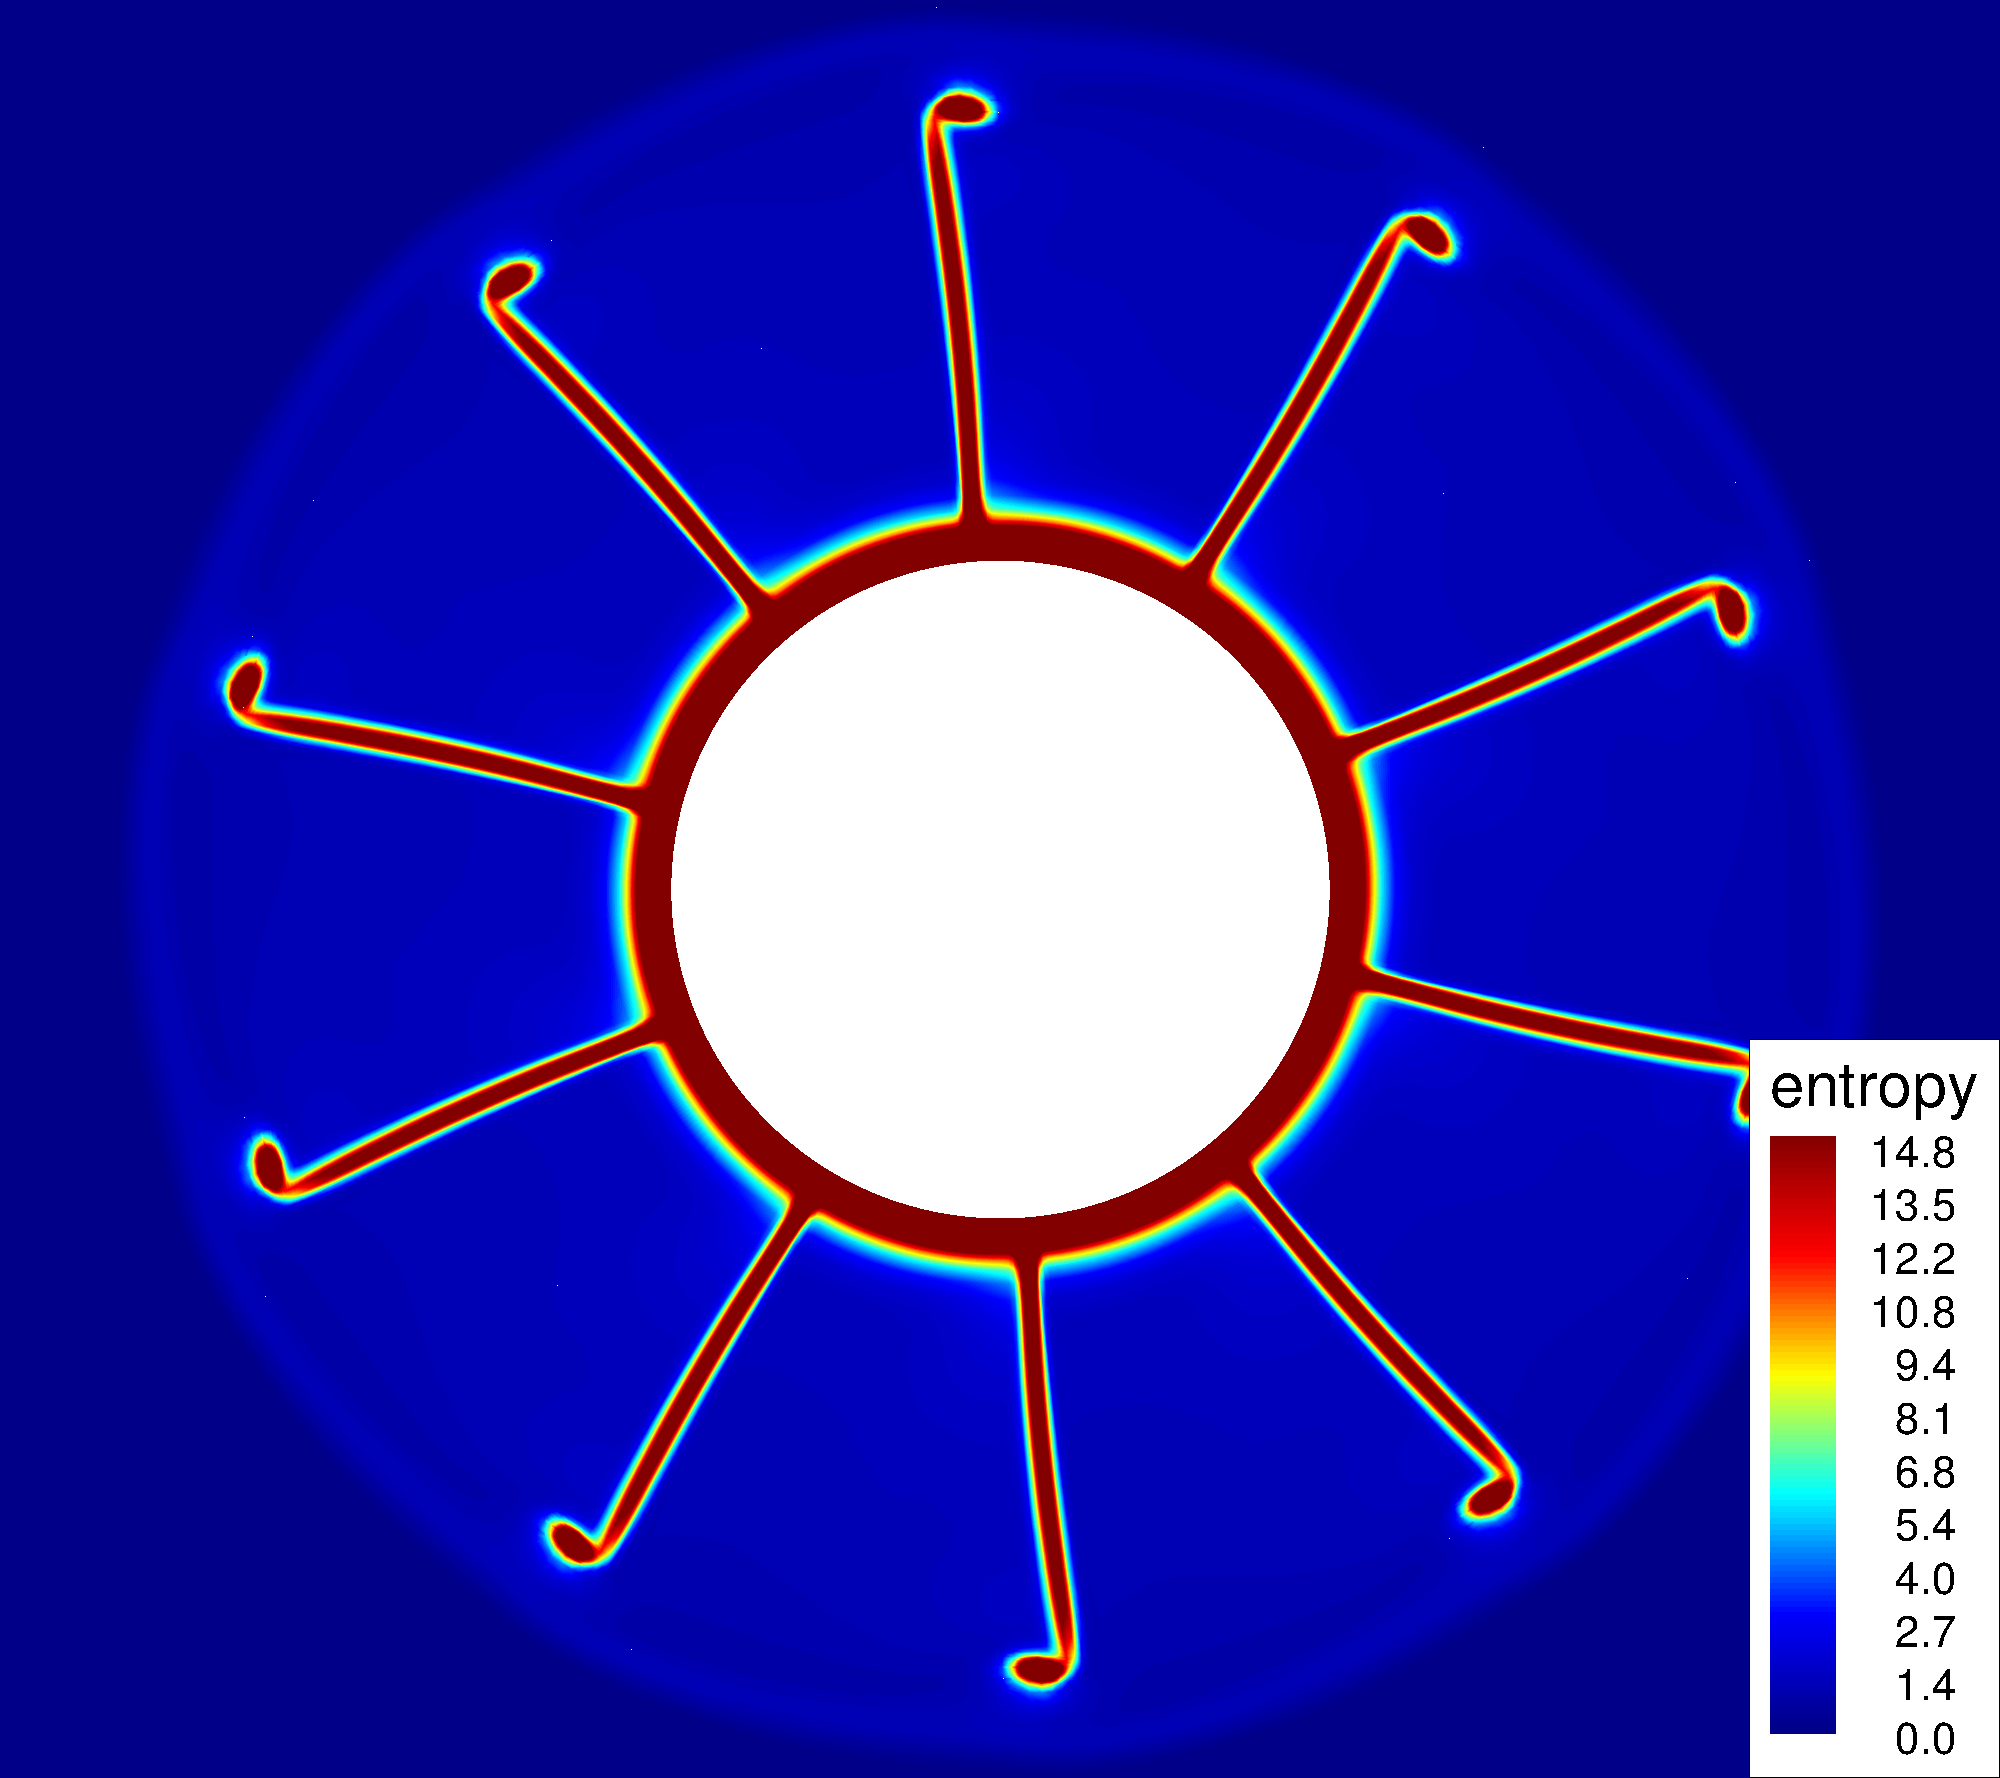
\includegraphics[width=.35\textwidth]{DREAM_HS_RANS_roe2_sa_slice_x_rear_1_entropy.png}}
  \subfigure[$P6$]{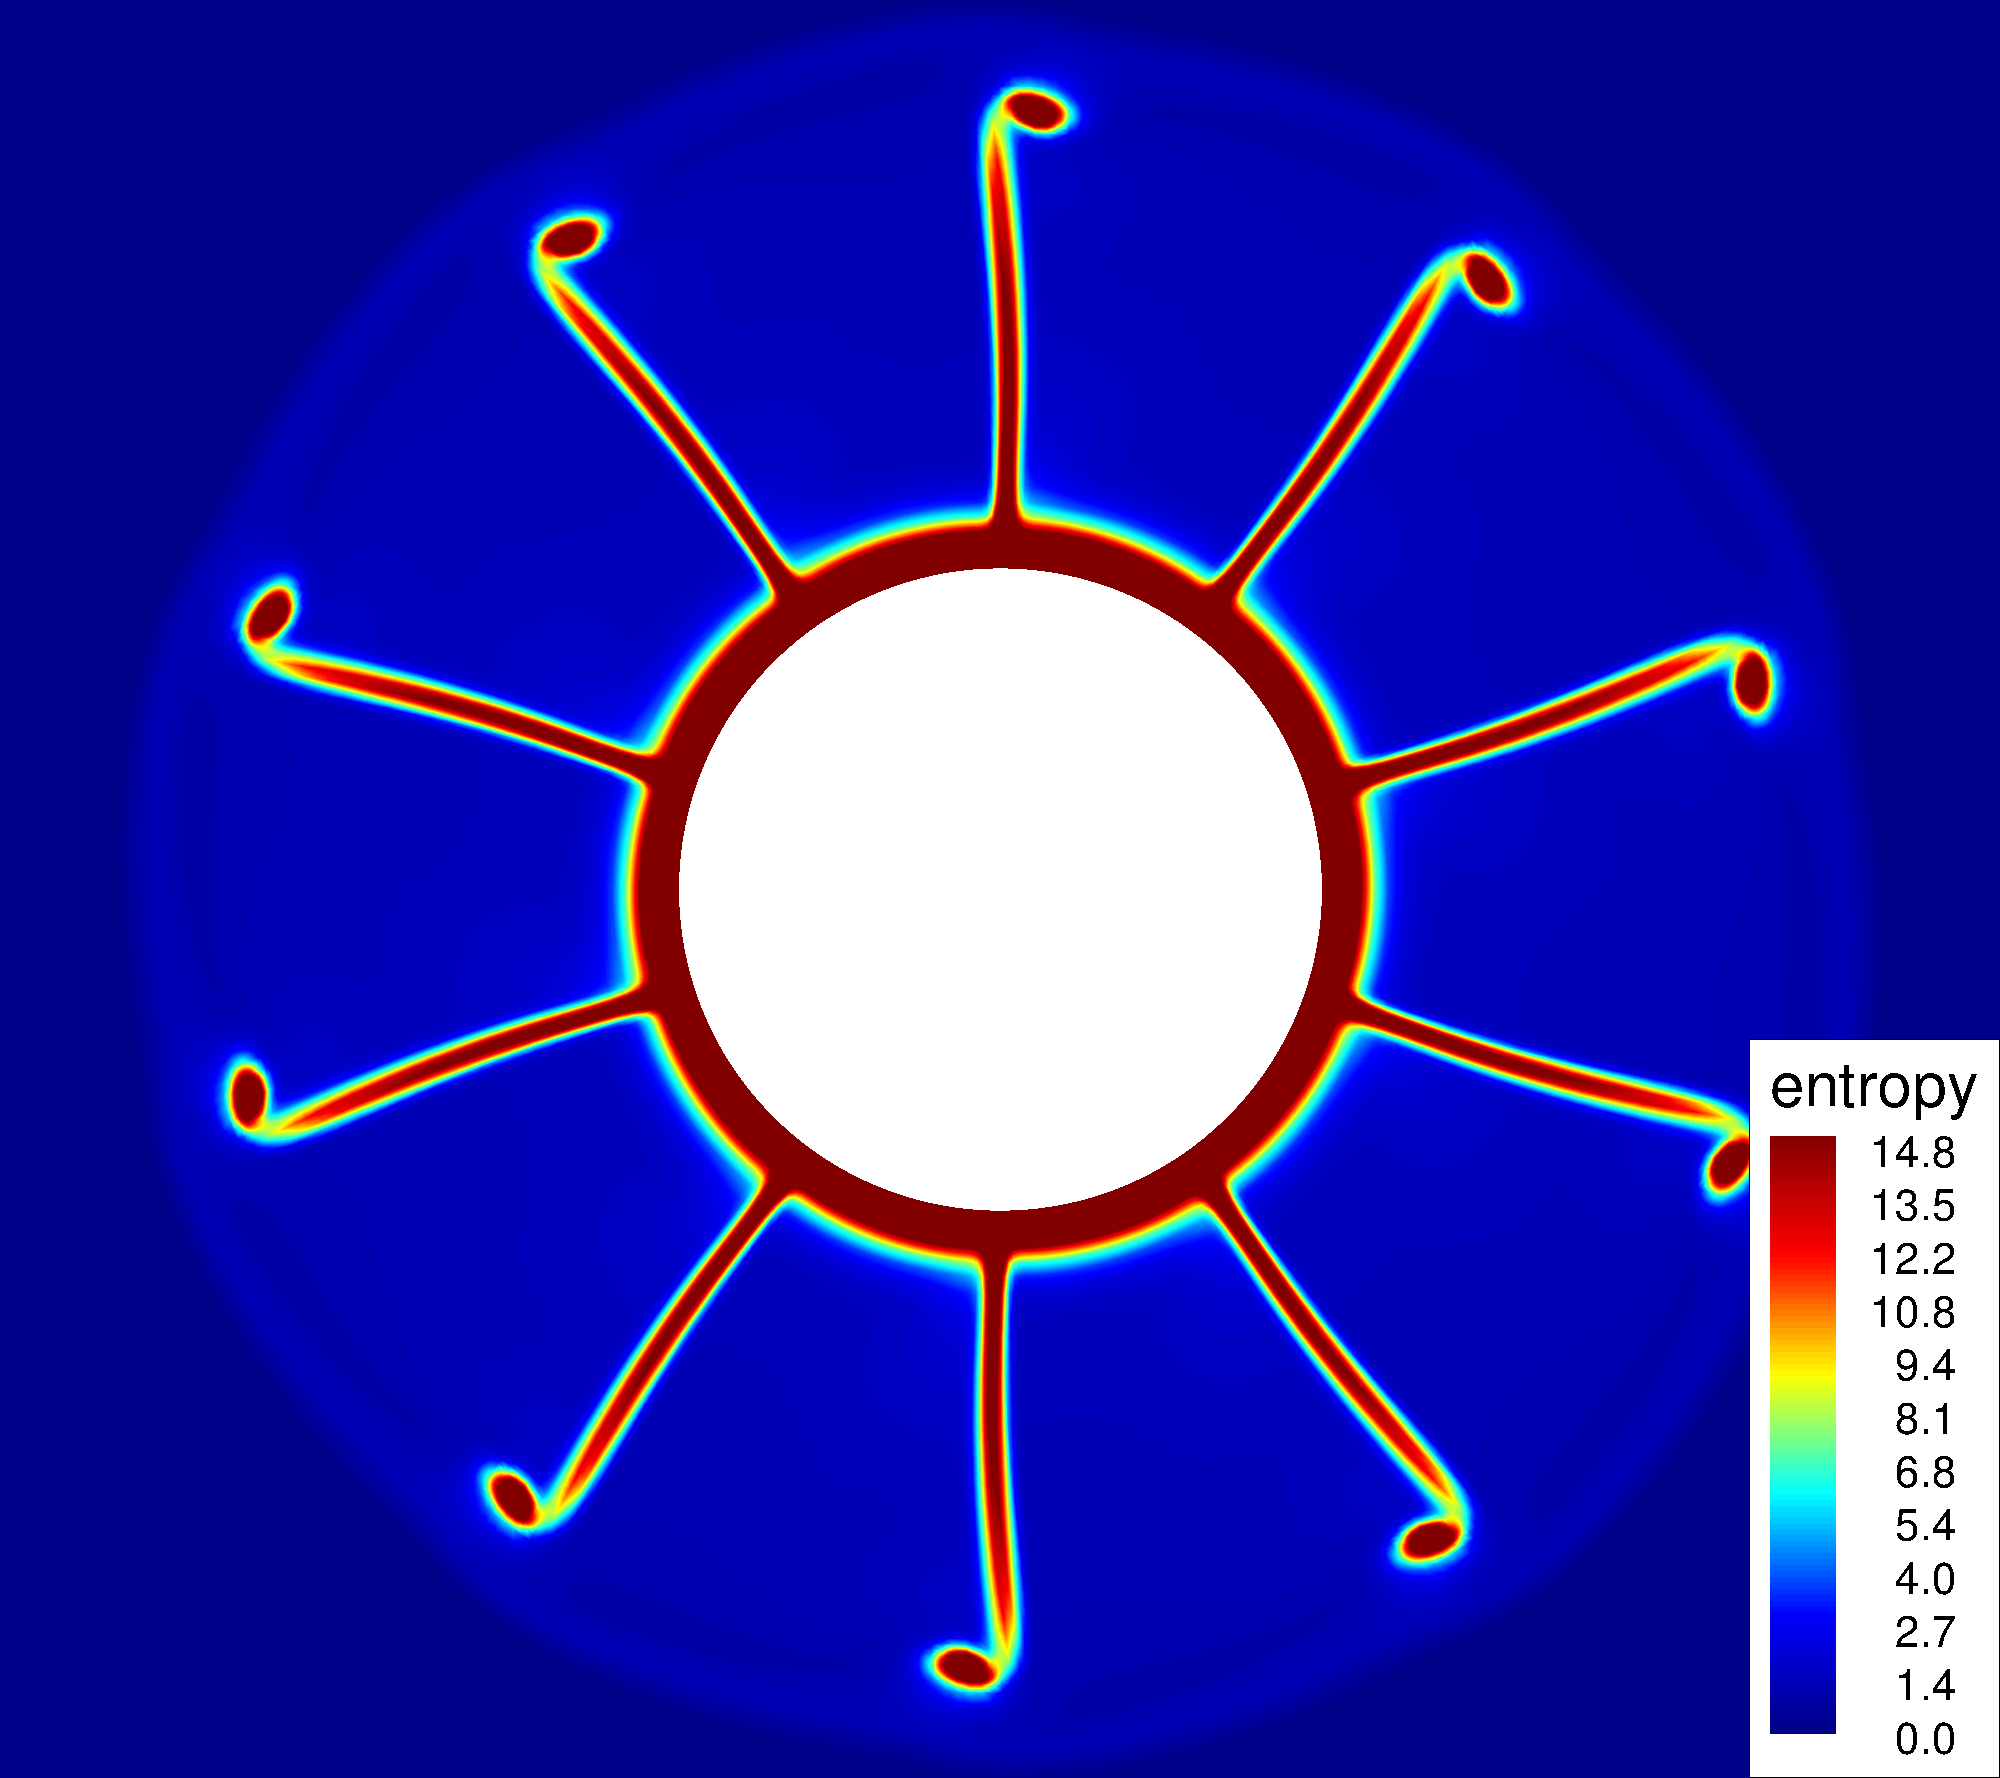
\includegraphics[width=.35\textwidth]{DREAM_HS_RANS_roe2_sa_slice_x_rear_2_entropy.png}}
  \caption{High-speed isolated configuration: axial cut of entropy.}
   \label{fig:dream_HS_steady_entropy}
\end{figure}